\documentclass[10pt,fleqn]{article} % Default font size and left-justified equations
\usepackage[%
    pdftitle={Modélisation systèmes multiphysiques : Modélisation linéaire et non linéaire},
    pdfauthor={Xavier Pessoles}]{hyperref}
    
%%%%%%%%%%%%%%%%%%%%%%%%%%%%%%%%%%%%%%%%%
% Original author:
% Mathias Legrand (legrand.mathias@gmail.com) with modifications by:
% Vel (vel@latextemplates.com)
% License:
% CC BY-NC-SA 3.0 (http://creativecommons.org/licenses/by-nc-sa/3.0/)
%%%%%%%%%%%%%%%%%%%%%%%%%%%%%%%%%%%%%%%%%

%----------------------------------------------------------------------------------------
%	VARIOUS REQUIRED PACKAGES AND CONFIGURATIONS
%----------------------------------------------------------------------------------------

%\usepackage[top=2.5cm,bottom=2cm,left=2cm,right=2cm,headsep=40pt,a4paper]{geometry} % Page margins
\usepackage[top=2cm,bottom=2cm,left=2cm,right=2cm,a4paper]{geometry} % Page margins

\usepackage{graphicx} % Required for including pictures

\usepackage{lipsum} % Inserts dummy text

\usepackage{tikz} % Required for drawing custom shapes

\usepackage[francais]{babel} % English language/hyphenation
\frenchbsetup{StandardLists=true} % Pour éviter la collision babel enumitem pour les listes

\usepackage{enumitem} % Customize lists
\setlist{nolistsep} % Reduce spacing between bullet points and numbered lists

\usepackage{booktabs} % Required for nicer horizontal rules in tables

\usepackage{xcolor} % Required for specifying colors by name
%\definecolor{ocre}{RGB}{243,102,25} % Define the orange color used for highlighting throughout the book
 \definecolor{ocre}{RGB}{49,133,156} % Couleur ''bleue''
\definecolor{violetf}{RGB}{112,48,160} % Couleur ''violet''
\usepackage{enumitem}
\usepackage{pifont} % Pour les dinglist
\usepackage{multicol}
\usepackage{array} % Centrage vertical dans les tableaux
\usepackage{schemabloc}

%----------------------------------------------------------------------------------------
%	FONTS
%----------------------------------------------------------------------------------------
\usepackage{bm}
\usepackage{multicol}
\usepackage{siunitx}
\sisetup{output-decimal-marker = {,}}


\usepackage{avant} % Use the Avantgarde font for headings
%\usepackage{times} % Use the Times font for headings
%\usepackage{mathptmx} % Use the Adobe Times Roman as the default text font together with math symbols from the Sym­bol, Chancery and Com­puter Modern fonts
\usepackage[adobe-utopia]{mathdesign}
\usepackage{microtype} % Slightly tweak font spacing for aesthetics
\usepackage[utf8]{inputenc} % Required for including letters with accents
\usepackage[T1]{fontenc} % Use 8-bit encoding that has 256 glyphs

%----------------------------------------------------------------------------------------
%	BIBLIOGRAPHY AND INDEX
%----------------------------------------------------------------------------------------

%\usepackage[style=alphabetic,citestyle=numeric,sorting=nyt,sortcites=true,autopunct=true,babel=hyphen,hyperref=true,abbreviate=false,backref=true,backend=biber]{biblatex}
\usepackage[style=alphabetic,citestyle=numeric,sorting=nyt,sortcites=true,autopunct=true,hyperref=true,abbreviate=false,backref=true,backend=biber]{biblatex}
\addbibresource{bibliography.bib} % BibTeX bibliography file
\defbibheading{bibempty}{}

\usepackage{calc} % For simpler calculation - used for spacing the index letter headings correctly
\usepackage{makeidx} % Required to make an index
\makeindex % Tells LaTeX to create the files required for indexing

%----------------------------------------------------------------------------------------
%	MAIN TABLE OF CONTENTS
%----------------------------------------------------------------------------------------

\usepackage{titletoc} % Required for manipulating the table of contents

\setcounter{tocdepth}{2}     % Dans la table des matieres
\setcounter{secnumdepth}{2}

\contentsmargin{0cm} % Removes the default margin

% Part text styling
\titlecontents{part}[0cm]
{\addvspace{20pt}\centering\large\bfseries}
{}
{}
{}

% Chapter text styling
\titlecontents{chapter}[1.25cm] % Indentation
{\addvspace{12pt}\large\sffamily\bfseries} % Spacing and font options for chapters
{\color{ocre!60}\contentslabel[\Large\thecontentslabel]{1.25cm}\color{ocre}} % Chapter number
{\color{ocre}}  
{\color{ocre!60}\normalsize\;\titlerule*[.5pc]{.}\;\thecontentspage} % Page number

% Section text styling
\titlecontents{section}[1.25cm] % Indentation
{\addvspace{3pt}\sffamily\bfseries} % Spacing and font options for sections
{\color{ocre!60}\contentslabel[\thecontentslabel]{1.25cm} \color{ocre}} % Section number
{\color{ocre}}
{\hfill\color{ocre!60}\thecontentspage} % Page number
[]

% Subsection text styling
\titlecontents{subsection}[1.25cm] % Indentation
{\addvspace{1pt}\sffamily\small} % Spacing and font options for subsections
{\contentslabel[\thecontentslabel]{1.25cm}} % Subsection number
{}
{\ \titlerule*[.5pc]{.}\;\thecontentspage} % Page number
[]


% Subsection text styling
\titlecontents{subsubsection}[1.25cm] % Indentation
{\addvspace{1pt}\sffamily\small} % Spacing and font options for subsections
{\contentslabel[\thecontentslabel]{1.25cm}} % Subsection number
{}
{\ \titlerule*[.5pc]{.}\;\thecontentspage} % Page number
[]

% List of figures
\titlecontents{figure}[0em]
{\addvspace{-5pt}\sffamily}
{\thecontentslabel\hspace*{1em}}
{}
{\ \titlerule*[.5pc]{.}\;\thecontentspage}
[]

% List of tables
\titlecontents{table}[0em]
{\addvspace{-5pt}\sffamily}
{\thecontentslabel\hspace*{1em}}
{}
{\ \titlerule*[.5pc]{.}\;\thecontentspage}
[]

%----------------------------------------------------------------------------------------
%	MINI TABLE OF CONTENTS IN PART HEADS
%----------------------------------------------------------------------------------------

% Chapter text styling
\titlecontents{lchapter}[0em] % Indenting
{\addvspace{15pt}\large\sffamily\bfseries} % Spacing and font options for chapters
{\color{ocre}\contentslabel[\Large\thecontentslabel]{1.25cm}\color{ocre}} % Chapter number
{}  
{\color{ocre}\normalsize\sffamily\bfseries\;\titlerule*[.5pc]{.}\;\thecontentspage} % Page number

% Section text styling
\titlecontents{lsection}[0em] % Indenting
{\sffamily\small} % Spacing and font options for sections
{\contentslabel[\thecontentslabel]{1.25cm}} % Section number
{}
{}

% Subsection text styling
\titlecontents{lsubsection}[.5em] % Indentation
{\normalfont\footnotesize\sffamily} % Font settings
{}
{}
{}

%----------------------------------------------------------------------------------------
%	PAGE HEADERS
%----------------------------------------------------------------------------------------

\usepackage{fancyhdr} % Required for header and footer configuration



\pagestyle{fancy}
 \renewcommand{\headrulewidth}{0pt}
 \fancyhead{}
 
 % ENTETES de page
 \fancyhead[L]{%
 \begin{tikzpicture}[overlay]
\node(logo) at (1,0)
    {
\includegraphics[width=2cm]{logo_lycee.png}};
\end{tikzpicture}
 %\noindent\begin{minipage}[c]{2.6cm}%
 %
\includegraphics[width=2cm]{logo_lycee.png}%
 %\end{minipage}
}

\fancyhead[C]{\rule{8cm}{.5pt}}

 \fancyhead[R]{%
 \noindent\begin{minipage}[c]{3cm}
 \begin{flushright}
 \footnotesize{\textit{\textsf{\xxtete}}}%
 \end{flushright}
 \end{minipage}
}

 \fancyfoot{}
 % PIEDS de page
\fancyfoot[C]{\rule{12cm}{.5pt}}
\renewcommand{\footrulewidth}{0.2pt}
\fancyfoot[C]{\footnotesize{\bfseries \thepage}}
\fancyfoot[L]{ 
\begin{minipage}[c]{.4\linewidth}
\noindent\footnotesize{{\xxauteur}}
\end{minipage}}

\fancyfoot[R]{\footnotesize{\xxpied}
\ifthenelse{\isodd{\value{page}}}{
\begin{tikzpicture}[overlay]
\node[shape=rectangle, 
      rounded corners = .25 cm,
	  draw= ocre,
	  line width=2pt, 
	  fill = ocre!10,
	  minimum width  = 2.5cm,
	  minimum height = 3cm,] at (\xxposongletx,\xxposonglety) {};
\node at (\xxposonglettext,\xxposonglety) {\rotatebox{90}{\textbf{\large\color{ocre}{\xxonglet}}}};
%{};
\end{tikzpicture}}{}
}



%
%
%
% Removes the header from odd empty pages at the end of chapters
\makeatletter
%\renewcommand{\cleardoublepage}{
%\clearpage\ifodd\c@page\else
%\hbox{}
%\vspace*{\fill}
%\thispagestyle{empty}
%\newpage
%\fi}

%\fancypagestyle{plain}{%
%\fancyhf{} % vide l’en-tête et le pied~de~page.
%%\fancyfoot[C]{\bfseries \thepage} % numéro de la page en cours en gras
%% et centré en pied~de~page.
%\fancyfoot[R]{\footnotesize{\xxpied}}
%\fancyfoot[C]{\rule{12cm}{.5pt}}
%\renewcommand{\footrulewidth}{0.2pt}
%\fancyfoot[C]{\footnotesize{\bfseries \thepage}}
%\fancyfoot[L]{ 
%\begin{minipage}[c]{.4\linewidth}
%\noindent\footnotesize{{\xxauteur}}
%\end{minipage}}}

\fancypagestyle{plain}{%
\fancyhf{} % vide l’en-tête et le pied~de~page.
\fancyfoot[C]{\rule{12cm}{.5pt}}
\renewcommand{\footrulewidth}{0.2pt}
\fancyfoot[C]{\footnotesize{\bfseries \thepage}}
\fancyfoot[L]{ 
\begin{minipage}[c]{.4\linewidth}
\noindent\footnotesize{{\xxauteur}}
\end{minipage}}
\fancyfoot[R]{\footnotesize{\xxpied}}
}




%----------------------------------------------------------------------------------------
%	THEOREM STYLES
%----------------------------------------------------------------------------------------

% Conflit avec la police adobe
%\usepackage{amsmath,amsfonts,amssymb,amsthm} % For math equations, theorems, symbols, etc
\usepackage{amsmath,amsthm}

\newcommand{\intoo}[2]{\mathopen{]}#1\,;#2\mathclose{[}}
\newcommand{\ud}{\mathop{\mathrm{{}d}}\mathopen{}}
\newcommand{\intff}[2]{\mathopen{[}#1\,;#2\mathclose{]}}
%\newtheorem{notation}{Notation}[chapter]
\newtheorem{notation}{Notation}[section]

% Boxed/framed environments
\newtheoremstyle{ocrenumbox}% % Theorem style name
{0pt}% Space above
{0pt}% Space below
{\normalfont}% % Body font
{}% Indent amount
{\small\bf\sffamily\color{ocre}}% % Theorem head font
{\;}% Punctuation after theorem head
{0.25em}% Space after theorem head
{\small\sffamily\color{ocre}\thmname{#1}\nobreakspace\thmnumber%{\@ifnotempty{#1}{}\@upn{#2}}% Theorem text (e.g. Theorem 2.1)
\thmnote{\nobreakspace\the\thm@notefont\sffamily\bfseries\color{black}---\nobreakspace#3.}} % Optional theorem note
\renewcommand{\qedsymbol}{$\blacksquare$}% Optional qed square


% Boite pour les corriges
\newtheoremstyle{correctionbox}% % Theorem style name
{0pt}% Space above
{0pt}% Space below
{\normalfont}% % Body font
{}% Indent amount
{\small\bf\sffamily\color{violet}}% % Theorem head font
{\;}% Punctuation after theorem head
{0.25em}% Space after theorem head
{\small\sffamily\color{ocre}\thmname{#1}\nobreakspace\thmnumber%{\@ifnotempty{#1}{}\@upn{#2}}% Theorem text (e.g. Theorem 2.1)
\thmnote{\nobreakspace\the\thm@notefont\sffamily\bfseries\color{black}---\nobreakspace#3.}} % Optional theorem note
\renewcommand{\qedsymbol}{$\blacksquare$}% Optional qed square



\newtheoremstyle{blacknumex}% Theorem style name
{5pt}% Space above
{5pt}% Space below
{\normalfont}% Body font
{} % Indent amount
{\small\bf\sffamily}% Theorem head font
{\;}% Punctuation after theorem head
{0.25em}% Space after theorem head
{\small\sffamily{\tiny\ensuremath{\blacksquare}}\nobreakspace\thmname{#1}\nobreakspace\thmnumber%{\@ifnotempty{#1}{}\@upn{#2}}% Theorem text (e.g. Theorem 2.1)
\thmnote{\nobreakspace\the\thm@notefont\sffamily\bfseries---\nobreakspace#3.}}% Optional theorem note

\newtheoremstyle{blacknumbox} % Theorem style name
{0pt}% Space above
{0pt}% Space below
{\normalfont}% Body font
{}% Indent amount
{\small\bf\sffamily}% Theorem head font
{\;}% Punctuation after theorem head
{0.25em}% Space after theorem head
{\small\sffamily\thmname{#1}\nobreakspace 
\thmnote{\nobreakspace\the\thm@notefont\sffamily\bfseries---\nobreakspace#3.}}% Optional theorem note

% Non-boxed/non-framed environments
\newtheoremstyle{ocrenum}% % Theorem style name
{5pt}% Space above
{5pt}% Space below
{\normalfont}% % Body font
{}% Indent amount
{\small\bf\sffamily\color{ocre}}% % Theorem head font
{\;}% Punctuation after theorem head
{0.25em}% Space after theorem head
{\small\sffamily\color{ocre}\thmname{#1}\nobreakspace%\thmnumber{\@ifnotempty{#1}{}\@upn{#2}}% Theorem text (e.g. Theorem 2.1)
\thmnote{\nobreakspace\the\thm@notefont\sffamily\bfseries\color{black}---\nobreakspace#3.}} % Optional theorem note
\renewcommand{\qedsymbol}{$\blacksquare$}% Optional qed square
\makeatother

% Environnement pour les titres de parties
\newtheoremstyle{partiebox} 
{0pt}% Space above
{0pt}% Space below
{\normalfont}% Body font
{}% Indent amount
{\small\bf\sffamily}% Theorem head font
{\;}% Punctuation after theorem head
{0.25em}% Space after theorem head




% Defines the theorem text style for each type of theorem to one of the three styles above
\newcounter{dummy} 
\numberwithin{dummy}{section}
\theoremstyle{ocrenumbox}
%\newtheorem{theoremeT}[dummy]{Théorème}
\newtheorem{theoremeT}[dummy]{Théorème}
\newtheorem{resultatT}[dummy]{Résultat}
\newtheorem{savoirT}[dummy]{Savoir}
\newtheorem{methodeT}[dummy]{Méthode}
\newtheorem{objectifT}[dummy]{Objectif}
%\newtheorem{problem}{Problem}[chapter]
\newtheorem{problem}{Problem}[section]
%\newtheorem{exerciseT}{Exercise}[chapter]
\newtheorem{exerciseT}{Exercice}[section]

\theoremstyle{blacknumex}
%\newtheorem{exampleT}{Example}[chapter]
\newtheorem{exempleT}{Exemple}[section]
\newtheorem{termT}{Terminal\\}[section]
\newtheorem{pyT}{Python\\}[section]
\newtheorem{sciT}{Scilab\\}[section]
\newtheorem{pseudoT}{Pseudo Code\\}[section]
\newtheorem{sqlT}{SQL\\}[section]

\theoremstyle{blacknumbox}
%\newtheorem{vocabulary}{Vocabulary}[chapter]
\newtheorem{vocabulary}{Vocabulaire}[section]
%\newtheorem{definitionT}{Definition}[section]
\newtheorem{definitionT}{Définition}[section]
\newtheorem{propT}{Propriété}[section]
\newtheorem{rappelT}{Rappel}[section]
\newtheorem{demoT}{Démonstration}[section]
\newtheorem{corollaryT}[dummy]{Corollaire}
\newtheorem{hypoT}{Hypothèse(s)}

\theoremstyle{ocrenum}
\newtheorem{proposition}[dummy]{Proposition}

\theoremstyle{partiebox}
\newtheorem{titrepartieT}[]{}
\newtheorem{titrechapitreT}[]{}

\theoremstyle{correctionbox}
\newtheorem{correctionT}[dummy]{\color{violet}{Correction}}

%----------------------------------------------------------------------------------------
%	DEFINITION OF COLORED BOXES
%----------------------------------------------------------------------------------------

\RequirePackage[framemethod=tikz]{mdframed} % Required for creating the theorem, definition, exercise and corollary boxes

% Theorem box
\newmdenv[skipabove=7pt,
skipbelow=7pt,
backgroundcolor=ocre!10,
linecolor=ocre,
innerleftmargin=5pt,
innerrightmargin=5pt,
innertopmargin=5pt,
leftmargin=0cm,
rightmargin=0cm,
innerbottommargin=5pt]{tBox}


% Correction
\newmdenv[skipabove=7pt,
skipbelow=7pt,
backgroundcolor=violet!10,
linecolor=violet,
innerleftmargin=5pt,
innerrightmargin=5pt,
innertopmargin=5pt,
leftmargin=0cm,
rightmargin=0cm,
innerbottommargin=5pt]{coBox}


% Exercise box	  
\newmdenv[skipabove=7pt,
skipbelow=7pt,
rightline=false,
leftline=true,
topline=false,
bottomline=false,
backgroundcolor=ocre!10,
linecolor=ocre,
innerleftmargin=5pt,
innerrightmargin=5pt,
innertopmargin=5pt,
innerbottommargin=5pt,
leftmargin=0cm,
rightmargin=0cm,
linewidth=4pt]{eBox}	

% Definition box
\newmdenv[skipabove=7pt,
skipbelow=7pt,
rightline=false,
leftline=true,
topline=false,
bottomline=false,
backgroundcolor=ocre!10,
linecolor=ocre,
innerleftmargin=5pt,
innerrightmargin=5pt,
innertopmargin=0pt,
leftmargin=0cm,
rightmargin=0cm,
linewidth=4pt,
innerbottommargin=0pt]{dBox}	

% Demonstration box
\newmdenv[skipabove=7pt,
skipbelow=7pt,
rightline=false,
leftline=true,
topline=false,
bottomline=false,
%backgroundcolor=ocre!10,
linecolor=ocre,
innerleftmargin=5pt,
innerrightmargin=5pt,
innertopmargin=0pt,
leftmargin=0cm,
rightmargin=0cm,
linewidth=4pt,
innerbottommargin=0pt]{demoBox}	

% Corollary box
\newmdenv[skipabove=7pt,
skipbelow=7pt,
rightline=false,
leftline=true,
topline=false,
bottomline=false,
linecolor=gray,
backgroundcolor=black!5,
innerleftmargin=5pt,
innerrightmargin=5pt,
innertopmargin=5pt,
leftmargin=0cm,
rightmargin=0cm,
linewidth=4pt,
innerbottommargin=5pt]{cBox}


% Hypothèses
\newmdenv[skipabove=7pt,
skipbelow=7pt,
rightline=false,
leftline=true,
topline=false,
bottomline=false,
linecolor=gray,
backgroundcolor=black!5,
innerleftmargin=5pt,
innerrightmargin=5pt,
innertopmargin=5pt,
leftmargin=0cm,
rightmargin=0cm,
linewidth=4pt,
innerbottommargin=5pt]{hyBox}


% Boite pour le titre de la partie (pBox)
\newmdenv[skipabove=7pt,
skipbelow=7pt,
rightline=true,
leftline=false,
topline=false,
bottomline=false,
linecolor=ocre,
backgroundcolor=none,
innerleftmargin=5pt,
innerrightmargin=5pt,
innertopmargin=5pt,
leftmargin=0cm,
rightmargin=0cm,
linewidth=4pt,
innerbottommargin=5pt]{pBox}

% Boite pour le titre du chapitre (chBox)
\newmdenv[skipabove=7pt,
skipbelow=7pt,
rightline=false,
leftline=true,
topline=false,
bottomline=false,
linecolor=ocre,
%backgroundcolor=black!5,
innerleftmargin=5pt,
innerrightmargin=5pt,
innertopmargin=5pt,
leftmargin=0cm,
rightmargin=0cm,
linewidth=4pt,
innerbottommargin=5pt]{chBox}


% Boite pour les exemples
\newmdenv[skipabove=7pt,
skipbelow=7pt,
rightline=false,
leftline=true,
topline=false,
bottomline=false,
linecolor=gray,
backgroundcolor=white,
innerleftmargin=5pt,
innerrightmargin=5pt,
innertopmargin=5pt,
leftmargin=0cm,
rightmargin=0cm,
linewidth=4pt,
innerbottommargin=5pt]{exBox}

% Boite pour le terminal
\newmdenv[skipabove=7pt,
skipbelow=7pt,
rightline=false,
leftline=true,
topline=false,
bottomline=false,
linecolor=gray,
backgroundcolor=white,
innerleftmargin=5pt,
innerrightmargin=5pt,
innertopmargin=5pt,
leftmargin=0cm,
rightmargin=0cm,
linewidth=4pt,
innerbottommargin=5pt]{termBox}


% Boite pour Python
\newmdenv[skipabove=7pt,
skipbelow=7pt,
rightline=false,
leftline=true,
topline=false,
bottomline=false,
linecolor=gray,
backgroundcolor=white,
innerleftmargin=5pt,
innerrightmargin=5pt,
innertopmargin=0pt,
leftmargin=0cm,
rightmargin=0cm,
linewidth=4pt,
innerbottommargin=5pt]{pyBox}

% Boite pour scilab
\newmdenv[skipabove=7pt,
skipbelow=7pt,
rightline=false,
leftline=true,
topline=false,
bottomline=false,
linecolor=gray,
backgroundcolor=white,
innerleftmargin=5pt,
innerrightmargin=5pt,
innertopmargin=5pt,
leftmargin=0cm,
rightmargin=0cm,
linewidth=4pt,
innerbottommargin=5pt]{sciBox}


% Boite pour pseudo
\newmdenv[skipabove=7pt,
skipbelow=7pt,
rightline=false,
leftline=true,
topline=false,
bottomline=false,
linecolor=gray,
backgroundcolor=white,
innerleftmargin=5pt,
innerrightmargin=5pt,
innertopmargin=5pt,
leftmargin=0cm,
rightmargin=0cm,
linewidth=4pt,
innerbottommargin=5pt]{pseudoBox}

% Boite pour pseudo
\newmdenv[skipabove=7pt,
skipbelow=7pt,
rightline=false,
leftline=true,
topline=false,
bottomline=false,
linecolor=gray,
backgroundcolor=white,
innerleftmargin=5pt,
innerrightmargin=5pt,
innertopmargin=5pt,
leftmargin=0cm,
rightmargin=0cm,
linewidth=4pt,
innerbottommargin=5pt]{sqlBox}


% Creates an environment for each type of theorem and assigns it a theorem text style from the "Theorem Styles" section above and a colored box from above
\newenvironment{theorem}{\begin{tBox}\begin{theoremeT}}{\end{theoremeT}\end{tBox}}
\newenvironment{resultat}{\begin{tBox}\begin{resultatT}}{\end{resultatT}\end{tBox}}
\newenvironment{methode}{\begin{tBox}\begin{methodeT}}{\end{methodeT}\end{tBox}}
\newenvironment{savoir}{\begin{tBox}\begin{savoirT}}{\end{savoirT}\end{tBox}}
\newenvironment{obj}{\begin{tBox}\begin{objectifT}}{\end{objectifT}\end{tBox}}
\newenvironment{corrige}{\begin{coBox}\begin{correctionT}}{\end{correctionT}\end{coBox}}
\newenvironment{exercise}{\begin{eBox}\begin{exerciseT}}{\hfill{\color{ocre}\tiny\ensuremath{\blacksquare}}\end{exerciseT}\end{eBox}}				  
\newenvironment{exercice}{\begin{eBox}\begin{exerciseT}}{\hfill{\color{ocre}\tiny\ensuremath{\blacksquare}}\end{exerciseT}\end{eBox}}				  

\newenvironment{definition}{\begin{dBox}\begin{definitionT}}{\end{definitionT}\end{dBox}}
\newenvironment{prop}{\begin{dBox}\begin{propT}}{\end{propT}\end{dBox}}	
\newenvironment{rappel}{\begin{dBox}\begin{rappelT}}{\end{rappelT}\end{dBox}}	
\newenvironment{defi}{\begin{dBox}\begin{definitionT}}{\end{definitionT}\end{dBox}}	
\newenvironment{demo}{\begin{demoBox}\begin{demoT}}{\end{demoT}\end{demoBox}}	
%\newenvironment{exemple}{\begin{exempleT}}{\hfill{\tiny\ensuremath{\blacksquare}}\end{exempleT}}		
\newenvironment{corollary}{\begin{cBox}\begin{corollaryT}}{\end{corollaryT}\end{cBox}}
\newenvironment{hypo}{\begin{hyBox}\begin{hypoT}}{\end{hypoT}\end{hyBox}}	\newenvironment{exemple}{\begin{exBox}\begin{exempleT}}{\hfill{\tiny\ensuremath{\blacksquare}}\end{exempleT}\end{exBox}}	
\newenvironment{titrepartie}{\begin{pBox}\begin{titrepartieT}}{\end{titrepartieT}\end{pBox}}	
\newenvironment{titrechapitre}{\begin{chBox}\begin{titrechapitreT}}{\end{titrechapitreT}\end{chBox}}	

\newenvironment{term}{ \begin{termBox}\begin{termT}}{\end{termT}\end{termBox}}
\newenvironment{py}{ \begin{pyBox}\begin{pyT}}{\end{pyT}\end{pyBox}}
\newenvironment{sci}{ \begin{sciBox}\begin{sciT}}{\end{sciT}\end{sciBox}}
\newenvironment{pseudo}{ \begin{pseudoBox}\begin{pseudoT}}{\end{pseudoT}\end{pseudoBox}}
\newenvironment{envsql}{ \begin{sqlBox}\begin{sqlT}}{\end{sqlT}\end{sqlBox}}


%----------------------------------------------------------------------------------------
%	REMARK ENVIRONMENT
%----------------------------------------------------------------------------------------

\newenvironment{remark}{\par\vspace{10pt}\small % Vertical white space above the remark and smaller font size
\begin{list}{}{
\leftmargin=35pt % Indentation on the left
\rightmargin=25pt}\item\ignorespaces % Indentation on the right
\makebox[-2.5pt]{\begin{tikzpicture}[overlay]
\node[draw=ocre!60,line width=1pt,circle,fill=ocre!25,font=\sffamily\bfseries,inner sep=2pt,outer sep=0pt] at (-15pt,0pt){\textcolor{ocre}{R}};\end{tikzpicture}} % Orange R in a circle
\advance\baselineskip -1pt}{\end{list}\vskip5pt} % Tighter line spacing and white space after remark

\newenvironment{rem}{\par\vspace{10pt}\small % Vertical white space above the remark and smaller font size
\begin{list}{}{
\leftmargin=35pt % Indentation on the left
\rightmargin=25pt}\item\ignorespaces % Indentation on the right
\makebox[-2.5pt]{\begin{tikzpicture}[overlay]
\node[draw=ocre!60,line width=1pt,circle,fill=ocre!25,font=\sffamily\bfseries,inner sep=2pt,outer sep=0pt] at (-15pt,0pt){\textcolor{ocre}{R}};\end{tikzpicture}} % Orange R in a circle
\advance\baselineskip -1pt}{\end{list}\vskip5pt} % Tighter line spacing and white space after remark


\newenvironment{warn}{\par\vspace{10pt}\small % Vertical white space above the remark and smaller font size
\begin{list}{}{
\leftmargin=35pt % Indentation on the left
\rightmargin=25pt}\item\ignorespaces % Indentation on the right
\makebox[-2.5pt]{\begin{tikzpicture}[overlay]
\node[draw=red!60,line width=1pt,circle,fill=red!25,font=\sffamily\bfseries,inner sep=2pt,outer sep=0pt] at (-15pt,0pt){\textcolor{black}{!}};\end{tikzpicture}} % Point d'exclamation dans un cercle
\advance\baselineskip -1pt}{\end{list}\vskip5pt} % Tighter line spacing and white space after remark


%----------------------------------------------------------------------------------------
%	SECTION NUMBERING IN THE MARGIN
%----------------------------------------------------------------------------------------
\setcounter{secnumdepth}{3}
\setcounter{tocdepth}{2}



\makeatletter
\renewcommand{\@seccntformat}[1]{\llap{\textcolor{ocre}{\csname the#1\endcsname}\hspace{1em}}}                    
\renewcommand{\section}{\@startsection{section}{1}{\z@}
{-4ex \@plus -1ex \@minus -.4ex}
{1ex \@plus.2ex }
{\normalfont\large\sffamily\bfseries}}
\renewcommand{\subsection}{\@startsection {subsection}{2}{\z@}
{-3ex \@plus -0.1ex \@minus -.4ex}
{0.5ex \@plus.2ex }
{\normalfont\sffamily\bfseries}}
\renewcommand{\subsubsection}{\@startsection {subsubsection}{3}{\z@}
{-2ex \@plus -0.1ex \@minus -.2ex}
{.2ex \@plus.2ex }
{\normalfont\small\sffamily\bfseries}}                        
\renewcommand\paragraph{\@startsection{paragraph}{4}{\z@}
{-2ex \@plus-.2ex \@minus .2ex}
{.1ex}
{\normalfont\small\sffamily\bfseries}}

%----------------------------------------------------------------------------------------
%	PART HEADINGS
%----------------------------------------------------------------------------------------


%----------------------------------------------------------------------------------------
%	CHAPTER HEADINGS
%----------------------------------------------------------------------------------------

% \newcommand{\thechapterimage}{}%
% \newcommand{\chapterimage}[1]{\renewcommand{\thechapterimage}{#1}}%
% \def\@makechapterhead#1{%
% {\parindent \z@ \raggedright \normalfont
% \ifnum \c@secnumdepth >\m@ne
% \if@mainmatter
% \begin{tikzpicture}[remember picture,overlay]
% \node at (current page.north west)
% {\begin{tikzpicture}[remember picture,overlay]
% \node[anchor=north west,inner sep=0pt] at (0,0) {\includegraphics[width=\paperwidth]{\thechapterimage}};
% \draw[anchor=west] (\Gm@lmargin,-9cm) node [line width=2pt,rounded corners=15pt,draw=ocre,fill=white,fill opacity=0.5,inner sep=15pt]{\strut\makebox[22cm]{}};
% \draw[anchor=west] (\Gm@lmargin+.3cm,-9cm) node {\huge\sffamily\bfseries\color{black}\thechapter. #1\strut};
% \end{tikzpicture}};
% \end{tikzpicture}
% \else
% \begin{tikzpicture}[remember picture,overlay]
% \node at (current page.north west)
% {\begin{tikzpicture}[remember picture,overlay]
% \node[anchor=north west,inner sep=0pt] at (0,0) {\includegraphics[width=\paperwidth]{\thechapterimage}};
% \draw[anchor=west] (\Gm@lmargin,-9cm) node [line width=2pt,rounded corners=15pt,draw=ocre,fill=white,fill opacity=0.5,inner sep=15pt]{\strut\makebox[22cm]{}};
% \draw[anchor=west] (\Gm@lmargin+.3cm,-9cm) node {\huge\sffamily\bfseries\color{black}#1\strut};
% \end{tikzpicture}};
% \end{tikzpicture}
% \fi\fi\par\vspace*{270\p@}}}

%-------------------------------------------

\def\@makeschapterhead#1{%
\begin{tikzpicture}[remember picture,overlay]
\node at (current page.north west)
{\begin{tikzpicture}[remember picture,overlay]
\node[anchor=north west,inner sep=0pt] at (0,0) {\includegraphics[width=\paperwidth]{\thechapterimage}};
\draw[anchor=west] (\Gm@lmargin,-9cm) node [line width=2pt,rounded corners=15pt,draw=ocre,fill=white,fill opacity=0.5,inner sep=15pt]{\strut\makebox[22cm]{}};
\draw[anchor=west] (\Gm@lmargin+.3cm,-9cm) node {\huge\sffamily\bfseries\color{black}#1\strut};
\end{tikzpicture}};
\end{tikzpicture}
\par\vspace*{270\p@}}
\makeatother

%----------------------------------------------------------------------------------------
%	HYPERLINKS IN THE DOCUMENTS
%----------------------------------------------------------------------------------------


\hypersetup{hidelinks,backref=true,pagebackref=true,hyperindex=true,colorlinks=false,breaklinks=true,urlcolor= ocre,bookmarks=true,bookmarksopen=false,pdftitle={Title},pdfauthor={Author}}
\usepackage{bookmark}
\bookmarksetup{
open,
numbered,
addtohook={%
\ifnum\bookmarkget{level}=0 % chapter
\bookmarksetup{bold}%
\fi
\ifnum\bookmarkget{level}=-1 % part
\bookmarksetup{color=ocre,bold}%
\fi
}
}

%----------------------------------------------------------------------------------------
%	
%----------------------------------------------------------------------------------------

\newcommand{\thechapterimage}{}%
\newcommand{\chapterimage}[1]{\renewcommand{\thechapterimage}{#1}}%
\def\@makechapterhead#1{%
{\parindent \z@ \raggedright \normalfont
\begin{tikzpicture}[remember picture,overlay]
\node at (current page.north west)
{\begin{tikzpicture}[remember picture,overlay]
\node[anchor=north west,inner sep=0pt] at (0,0) {\includegraphics[width=\paperwidth]{\thechapterimage}};
%\draw[anchor=west] (\Gm@lmargin,-9cm) node [line width=2pt,rounded corners=15pt,draw=ocre,fill=white,fill opacity=0.5,inner sep=15pt]{\strut\makebox[22cm]{}};
%\draw[anchor=west] (\Gm@lmargin+.3cm,-9cm) node {\huge\sffamily\bfseries\color{black}\thechapter. #1\strut};
\end{tikzpicture}};
\end{tikzpicture}
\par\vspace*{270\p@}
}}

 \newcounter{exo}


\makeatletter             
\renewcommand{\subparagraph}{\@startsection{exo}{5}{\z@}%
                                    {-2ex \@plus-.2ex \@minus .2ex}%
                                    {0ex}%               
{\normalfont\bfseries Question \hspace{.7cm} }}
\makeatother
\renewcommand{\thesubparagraph}{\arabic{subparagraph}} 
\makeatletter


\usepackage{textcomp}

% Définition des booleéns
\newif\iffiche
\newif\ifprof
\newif\iftd
\newif\ifcours
\newif\ifnormal
\newif\ifdifficile
\newif\iftdifficile
\newif\ifcolle
\newif\iflivret
%%%%%%%%%%%%
% Définition des vecteurs 
%%%%%%%%%%%%
\newcommand{\vect}[1]{\overrightarrow{#1}}
\newcommand{\axe}[2]{\left(#1,\vect{#2}\right)}
\newcommand{\couple}[2]{\left(#1,\vect{#2}\right)}
\newcommand{\angl}[2]{\left(\vect{#1},\vect{#2}\right)}

\newcommand{\rep}[1]{\mathcal{R}_{#1}}
\newcommand{\quadruplet}[4]{\left(#1;#2,#3,#4 \right)}
\newcommand{\repere}[4]{\left(#1;\vect{#2},\vect{#3},\vect{#4} \right)}
\newcommand{\base}[3]{\left(\vect{#1},\vect{#2},\vect{#3} \right)}


\newcommand{\vx}[1]{\vect{x_{#1}}}
\newcommand{\vy}[1]{\vect{y_{#1}}}
\newcommand{\vz}[1]{\vect{z_{#1}}}

% d droit pour le calcul différentiel
\newcommand{\dd}{\text{d}}

\newcommand{\inertie}[2]{I_{#1}\left( #2\right)}
\newcommand{\matinertie}[7]{
\begin{pmatrix}
#1 & #6 & #5 \\
#6 & #2 & #4 \\
#5 & #4 & #3 \\
\end{pmatrix}_{#7}}
%%%%%%%%%%%%
% Définition des torseurs 
%%%%%%%%%%%%

\newcommand{\ec}[2]{%
\mathcal{E}_c\left(#1/#2\right)}

\newcommand{\pext}[3]{%
\mathcal{P}\left(#1\rightarrow#2/#3\right)}

\newcommand{\pint}[3]{%
\mathcal{P}\left(#1 \stackrel{\text{#3}}{\leftrightarrow} #2\right)}


 \newcommand{\torseur}[1]{%
\left\{{#1}\right\}
}

\newcommand{\torseurcin}[3]{%
\left\{\mathcal{#1} \left(#2/#3 \right) \right\}
}

\newcommand{\torseurci}[2]{%
\left\{\sigma \left(#1/#2 \right) \right\}
}
\newcommand{\torseurdyn}[2]{%
\left\{\mathcal{D} \left(#1/#2 \right) \right\}
}


\newcommand{\torseurstat}[3]{%
\left\{\mathcal{#1} \left(#2\rightarrow #3 \right) \right\}
}


 \newcommand{\torseurc}[8]{%
%\left\{#1 \right\}=
\left\{
{#1}
\right\}
 = 
\left\{%
\begin{array}{cc}%
{#2} & {#5}\\%
{#3} & {#6}\\%
{#4} & {#7}\\%
\end{array}%
\right\}_{#8}%
}

 \newcommand{\torseurcol}[7]{
\left\{%
\begin{array}{cc}%
{#1} & {#4}\\%
{#2} & {#5}\\%
{#3} & {#6}\\%
\end{array}%
\right\}_{#7}%
}

 \newcommand{\torseurl}[3]{%
%\left\{\mathcal{#1}\right\}_{#2}=%
\left\{%
\begin{array}{l}%
{#1} \\%
{#2} %
\end{array}%
\right\}_{#3}%
}

% Vecteur vitesse
 \newcommand{\vectv}[3]{%
\vect{V\left( {#1} \in {#2}/{#3}\right)}
}

% Vecteur force
\newcommand{\vectf}[2]{%
\vect{R\left( {#1} \rightarrow {#2}\right)}
}

% Vecteur moment stat
\newcommand{\vectm}[3]{%
\vect{\mathcal{M}\left( {#1}, {#2} \rightarrow {#3}\right)}
}




% Vecteur résultante cin
\newcommand{\vectrc}[2]{%
\vect{R_c \left( {#1}/ {#2}\right)}
}
% Vecteur moment cin
\newcommand{\vectmc}[3]{%
\vect{\sigma \left( {#1}, {#2} /{#3}\right)}
}


% Vecteur résultante dyn
\newcommand{\vectrd}[2]{%
\vect{R_d \left( {#1}/ {#2}\right)}
}
% Vecteur moment dyn
\newcommand{\vectmd}[3]{%
\vect{\delta \left( {#1}, {#2} /{#3}\right)}
}

% Vecteur accélération
 \newcommand{\vectg}[3]{%
\vect{\Gamma \left( {#1} \in {#2}/{#3}\right)}
}

% Vecteur omega
 \newcommand{\vecto}[2]{%
\vect{\Omega\left( {#1}/{#2}\right)}
}
% }$$\left\{\mathcal{#1} \right\}_{#2} =%
% \left\{%
% \begin{array}{c}%
%  #3 \\%
%  #4 %
% \end{array}%
% \right\}_{#5}}
\usepackage{multicol}
\usepackage{standalone}
\standaloneconfig{mode=buildnew}
\usepackage{siunitx}
\usepackage{wrapfig}
\fichetrue

%\fichefalse

\proftrue
\proffalse

\tdtrue
%\tdfalse

\courstrue
\coursfalse

\def\discipline{Sciences \\Industrielles de \\ l'Ingénieur}
\def\xxtete{Sciences Industrielles de l'Ingénieur}

\def\classe{MP}
\def\xxnumpartie{\textsf{Cy. 1 à 3}}
\def\xxpartie{Devoir Surveille 2}


\def\xxnumchapitre{9 novembre 2018 \vspace{.2cm}}
\def\xxchapitre{\hspace{.12cm}}%Modélisation multiphysique}


\def\xxtitreexo{\noindent Automate d’exploration de l’hémostase \\ \hspace{.4cm} Chargement et déchargement
des cargos porte-conteneurs }%Motorisation du moteur Haibike}
\def\xxsourceexo{\hspace{.2cm} CCP MP 2015 -- Centrale Supélec 2013}


\def\xxposongletx{2}
\def\xxposonglettext{1.45}
\def\xxposonglety{20}
%\def\xxonglet{Part. 1 -- Ch. 3}
\def\xxonglet{\textsf{Cy. 1 à 3}}

\def\xxactivite{DS 2}
\def\xxauteur{\textsl{Xavier Pessoles}}

\def\xxcompetences{%
\textsl{%
%\textbf{Savoirs et compétences :}\\
%Les sources sont associées par un \emph{hacheur série}. La détermination des grandeurs électriques associées à ce montage permet de conclure vis à vis du cahier des charges.
%\noindent \textbf{Résoudre :} à partir des modèles retenus :
%\begin{itemize}[label=\ding{112},font=\color{ocre}] 
%\item choisir une méthode de résolution analytique, graphique, numérique;
%\item mettre en \oe{}uvre une méthode de résolution.
%\end{itemize}
%\begin{itemize}[label=\ding{112},font=\color{ocre}] 
%\item \textit{Rés -- C1.1 :} Loi entrée sortie géométrique et cinématique -- Fermeture géométrique.
%\end{itemize}
%
%\noindent \textit{Mod2 -- C4.1 :} Représentation par schéma-blocs.
}}

\def\xxfigures{
%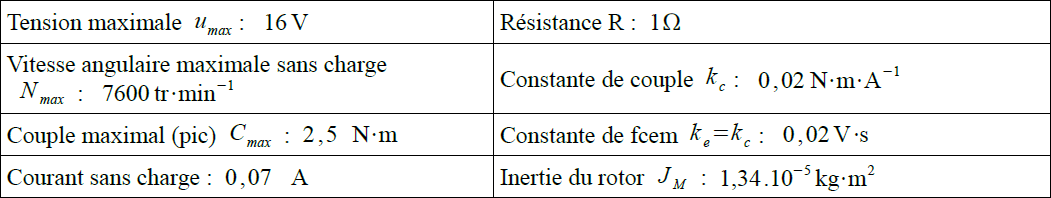
\includegraphics[width=.4\linewidth]{images/ccmp_06}
%\includegraphics[width=.4\linewidth]{images/ccs_00}
}%figues de la page de garde


\def\xxpied{%
%Cycle 01 -- Modéliser le comportement des systèmes multiphysiques\\
\xxactivite%
}

\setcounter{secnumdepth}{5}
%---------------------------------------------------------------------------

\usepackage{pgfplots}
\begin{document}
%\defimages{images}
%\chapterimage{png/Fond_Cin}
\pagestyle{empty}


%%%%%%%% PAGE DE GARDE COURS
\ifcours
% ==== BANDEAU DES TITRES ==== 
\begin{tikzpicture}[remember picture,overlay]
\node at (current page.north west)
{\begin{tikzpicture}[remember picture,overlay]
\node[anchor=north west,inner sep=0pt] at (0,0) {\includegraphics[width=\paperwidth]{\thechapterimage}};
\draw[anchor=west] (-2cm,-8cm) node [line width=2pt,rounded corners=15pt,draw=ocre,fill=white,fill opacity=0.6,inner sep=40pt]{\strut\makebox[22cm]{}};
\draw[anchor=west] (1cm,-8cm) node {\huge\sffamily\bfseries\color{black} %
\begin{minipage}{1cm}
\rotatebox{90}{\LARGE\sffamily\textsc{\color{ocre}\textbf{\xxnumpartie}}}
\end{minipage} \hfill
\begin{minipage}[c]{14cm}
\begin{titrepartie}
\begin{flushright}
\renewcommand{\baselinestretch}{1.1} 
\Large\sffamily\textsc{\textbf{\xxpartie}}
\renewcommand{\baselinestretch}{1} 
\end{flushright}
\end{titrepartie}
\end{minipage} \hfill
\begin{minipage}[c]{3.5cm}
{\large\sffamily\textsc{\textbf{\color{ocre} \discipline}}}
\end{minipage} 
 };
\end{tikzpicture}};
\end{tikzpicture}
% ==== FIN BANDEAU DES TITRES ==== 


% ==== ONGLET 
\begin{tikzpicture}[overlay]
\node[shape=rectangle, 
      rounded corners = .25 cm,
	  draw= ocre,
	  line width=2pt, 
	  fill = ocre!10,
	  minimum width  = 2.5cm,
	  minimum height = 3cm,] at (18.3cm,0) {};
\node at (17.7cm,0) {\rotatebox{90}{\textbf{\Large\color{ocre}{\classe}}}};
%{};
\end{tikzpicture}
% ==== FIN ONGLET 


\vspace{3.5cm}

\begin{tikzpicture}[remember picture,overlay]
\draw[anchor=west] (-2cm,-6cm) node {\huge\sffamily\bfseries\color{black} %
\begin{minipage}{2cm}
\begin{center}
\LARGE\sffamily\textsc{\color{ocre}\textbf{\xxactivite}}
\end{center}
\end{minipage} \hfill
\begin{minipage}[c]{15cm}
\begin{titrechapitre}
\renewcommand{\baselinestretch}{1.1} 
\Large\sffamily\textsc{\textbf{\xxnumchapitre}}

\Large\sffamily\textsc{\textbf{\xxchapitre}}
\vspace{.5cm}

\renewcommand{\baselinestretch}{1} 
\normalsize\normalfont
\xxcompetences
\end{titrechapitre}
\end{minipage}  };
\end{tikzpicture}
\vfill

\begin{flushright}
\begin{minipage}[c]{.3\linewidth}
\begin{center}
\xxfigures
\end{center}
\end{minipage}\hfill
\begin{minipage}[c]{.6\linewidth}
\startcontents
%\printcontents{}{1}{}
\printcontents{}{1}{}
\end{minipage}
\end{flushright}

\begin{tikzpicture}[remember picture,overlay]
\draw[anchor=west] (4.5cm,-.7cm) node {
\begin{minipage}[c]{.2\linewidth}
\begin{flushright}

\includegraphics[width=2cm]{logoCC}
\end{flushright}
\end{minipage}
\begin{minipage}[c]{.2\linewidth}
\textsl{\xxauteur} \\
\textsl{\classe}
\end{minipage}
 };
\end{tikzpicture}

\newpage
\pagestyle{fancy}

%\newpage
%\pagestyle{fancy}

\else
\fi
%% FIN PAGE DE GARDE DES COURS

%%%%%%%% PAGE DE GARDE TD
\iftd

% BANDEAU EXO
\iflivret % SI LIVRET ET TD
\begin{tikzpicture}[remember picture,overlay]
\draw[anchor=west] (-2cm,-3.3cm) node {\huge\sffamily\bfseries\color{black} %
\begin{minipage}{5cm}
\begin{center}
\LARGE\sffamily\color{ocre}\textbf{\textsc{\xxactivite}}

\begin{center}
\xxfigures
\end{center}

\end{center}
\end{minipage} \hfill
\begin{minipage}[c]{12cm}
\begin{titrechapitre}
\renewcommand{\baselinestretch}{1.1} 
\large\sffamily\textbf{\textsc{\xxtitreexo}}

\small\sffamily{\textbf{\textit{\color{black!70}\xxsourceexo}}}
\vspace{.5cm}

\renewcommand{\baselinestretch}{1} 
\normalsize\normalfont
\xxcompetences
\end{titrechapitre}
\end{minipage}};
\end{tikzpicture}
\else % ELSE NOT LIVRET
\begin{tikzpicture}[remember picture,overlay]
\draw[anchor=west] (-2cm,-3.5cm) node {\huge\sffamily\bfseries\color{black} %
\begin{minipage}{5cm}
\begin{center}
\LARGE\sffamily\color{ocre}\textbf{\textsc{\xxactivite}}

\begin{center}
\xxfigures
\end{center}

\end{center}
\end{minipage} \hfill
\begin{minipage}[c]{12cm}
\begin{titrechapitre}
\renewcommand{\baselinestretch}{1.1} 
\large\sffamily\textbf{\textsc{\xxtitreexo}}

\small\sffamily{\textbf{\textit{\color{black!70}\xxsourceexo}}}
\vspace{.5cm}

\renewcommand{\baselinestretch}{1} 
\normalsize\normalfont
\xxcompetences
\end{titrechapitre}
\end{minipage}};
\end{tikzpicture}

\fi

\else   % FIN IF TD
\fi


%%%%%%%% PAGE DE GARDE FICHE
\iffiche
\begin{tikzpicture}[remember picture,overlay]
\node at (current page.north west)
{\begin{tikzpicture}[remember picture,overlay]
\draw[anchor=west] (-2cm,\xxYCartouche) node [line width=2pt,rounded corners=15pt,draw=ocre,fill=white,fill opacity=0.6,inner sep=40pt]{\strut\makebox[22cm]{}};
\draw[anchor=west] (1cm,\xxYCartouche) node {\huge\sffamily\bfseries\color{black} %
\begin{minipage}{1cm}
\rotatebox{90}{\LARGE\sffamily\textsc{\color{ocre}\textbf{\xxnumpartie}}}
\end{minipage} \hfill
\begin{minipage}[c]{14cm}
\begin{titrepartie}
\begin{flushright}
\renewcommand{\baselinestretch}{1.1} 
\large\sffamily\textsc{\textbf{\xxpartie} \\} 

\vspace{.2cm}

\normalsize\sffamily\textsc{\textbf{\xxnumchapitre -- \xxchapitre}}
\renewcommand{\baselinestretch}{1} 
\end{flushright}
\end{titrepartie}
\end{minipage} \hfill
\begin{minipage}[c]{3.5cm}
{\large\sffamily\textsc{\textbf{\color{ocre} \discipline}}}
\end{minipage} 
 };
\end{tikzpicture}};
\end{tikzpicture}

\iflivret % SI LIVRET
\begin{tikzpicture}[overlay]
\node[shape=rectangle, 
      rounded corners = .25 cm,
	  draw= ocre,
	  line width=2pt, 
	  fill = ocre!10,
	  minimum width  = 2.5cm,
	  minimum height = 2.5cm,] at (18.5cm,\xxYongletGarde) {};
\node at (17.9cm,\xxYongletGarde) {\rotatebox{90}{\textsf{\textbf{\large\color{ocre}{\classe}}}}};
%{};
\end{tikzpicture}
\else  % SI PAS LIVRET
\iftd %% SI TD et PAS LIVRET
\begin{tikzpicture}[overlay]
\node[shape=rectangle, 
      rounded corners = .25 cm,
	  draw= ocre,
	  line width=2pt, 
	  fill = ocre!10,
	  minimum width  = 2.5cm,
	  minimum height = 2.5cm,] at (18.6cm,\xxYOnget) {}; %% 0.9 par défaut
\node at (18cm,\xxYOnget) {\rotatebox{90}{\textsf{\textbf{\large\color{ocre}{\classe}}}}};
%{};
\end{tikzpicture}

\else % FIN DU SI TD PAS LIVRET 
\begin{tikzpicture}[overlay]
\node[shape=rectangle, 
      rounded corners = .25 cm,
	  draw= ocre,
	  line width=2pt, 
	  fill = ocre!10,
	  minimum width  = 2.5cm,
%	  minimum height = 2.5cm,] at (18.5cm,1.1cm) {}; % \xxYOnget 0.5
	  minimum height = 2.5cm,] at (18.6cm,.5cm) {};
\node at (18cm,.5cm) {\rotatebox{90}{\textsf{\textbf{\large\color{ocre}{\classe}}}}};
%{};
\end{tikzpicture}
\fi
\fi
\else
\fi



\vspace{5cm}
\pagestyle{fancy}
\thispagestyle{plain}

\def\columnseprulecolor{\color{ocre}}
\setlength{\columnseprule}{0.4pt} 

%\defimages2{images}

%\begin{multicols}{2}
\section{Automate d’exploration de l’hémostase}
\subsection{Présentation du système}


\begin{minipage}[c]{.6\linewidth}
La société Stago est un laboratoire pharmaceutique de
l'industrie du Diagnostic In Vitro (DIV) entièrement
dédiée à l'exploration de l'hémostase et de la thrombose.
L'hémostase est le processus physiologique qui permet
d'interrompre le saignement pour éviter l'hémorragie.
L’objet de cette étude, le STA Compact, est un
automate de laboratoire destiné à l’analyse de
l’hémostase.
\end{minipage} \hfill
\begin{minipage}[c]{.35\linewidth}
\begin{center}
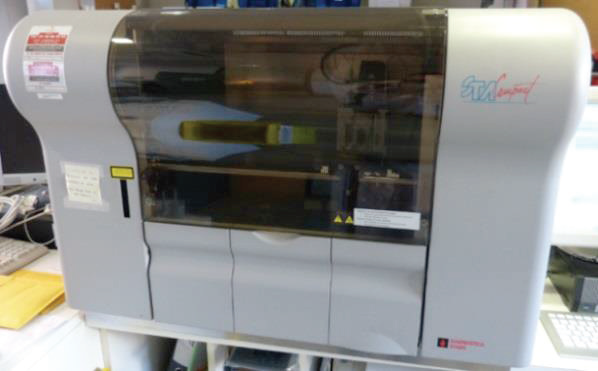
\includegraphics[width=\linewidth]{images/ccp_01}
\end{center}
\end{minipage} 

Les figures suivantes situent le STA Compact dans son environnement et précisent ses fonctions.

\begin{center}
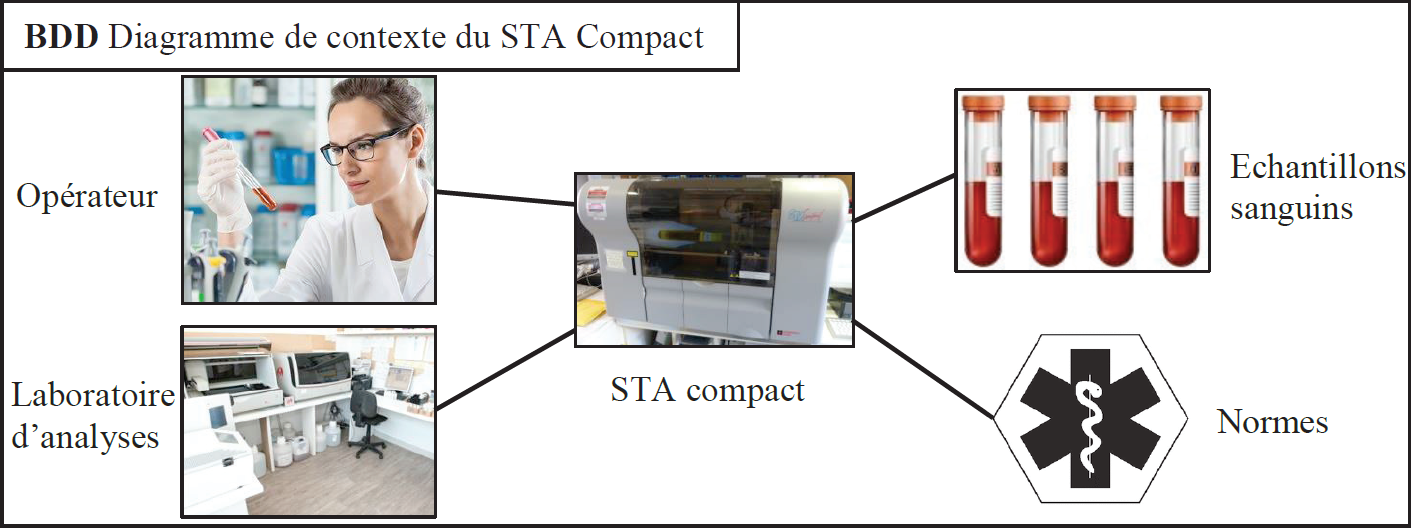
\includegraphics[width=.8\linewidth]{images/ccp_02}
\end{center}

\begin{center}
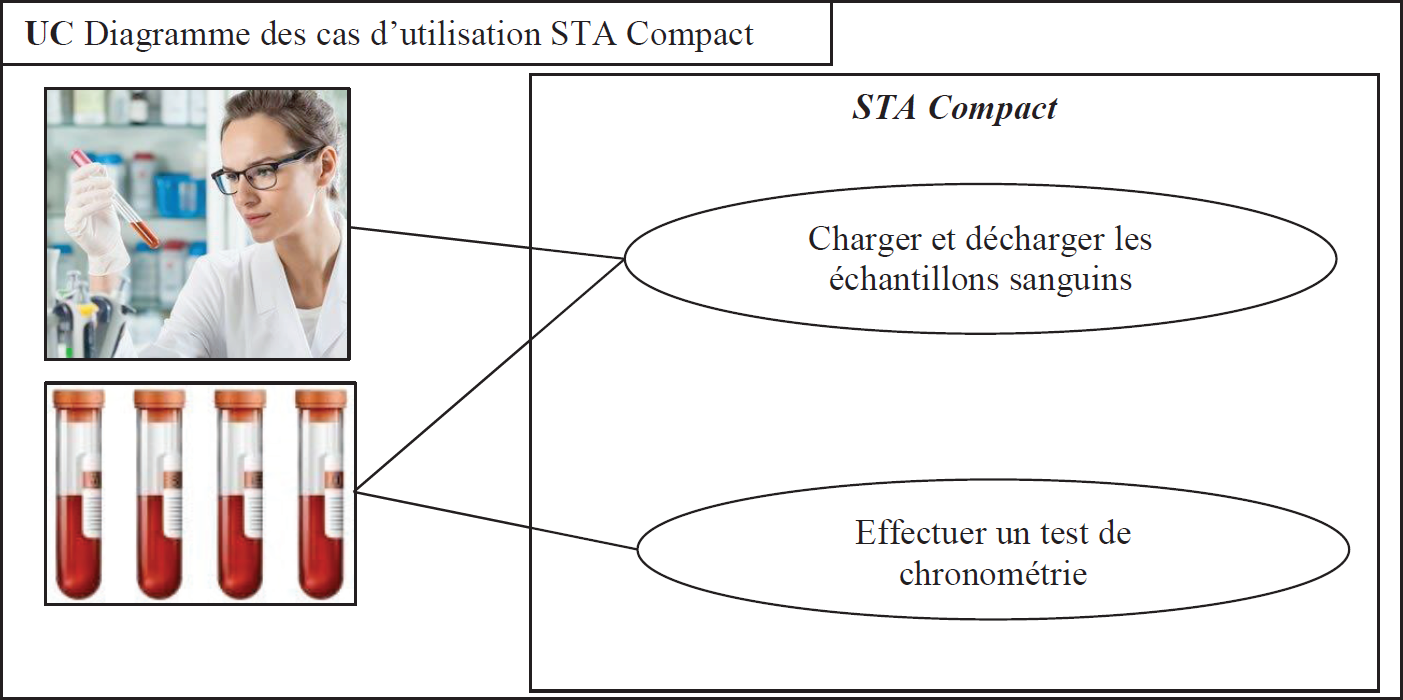
\includegraphics[width=.8\linewidth]{images/ccp_03}
\end{center}

Le STA Compact permet de réaliser, entre autre, des tests de chronométrie afin de mesurer un
temps de coagulation.

Le principe du test de chronométrie est le suivant :
\begin{itemize}
\item une dose de réactif est mélangée à une dose de plasma sanguin précédemment étuvée dans
une cuvette contenant une bille ;
\item l’ensemble est chauffé alors que la bille est mise en oscillation dans le mélange par un
champ magnétique ;
\item on mesure l’amplitude de l’oscillation qui diminue sensiblement lors d’une variation de
viscosité du mélange sang-réactif ;
\item le temps écoulé jusqu’à la diminution des oscillations donne le temps de coagulation.
\end{itemize}

\subsection{Analyse de l’exigence 3.3 « Mettre la bille en oscillation »}
\begin{obj}
Déterminer la pulsation optimale des bobines motrices.
\end{obj}

\subsubsection{Mise en situation}
Le principe de la chronométrie consiste à mesurer la variation de l’amplitude d’oscillation d’une
bille placée dans la cuvette de mesure.

\begin{center}
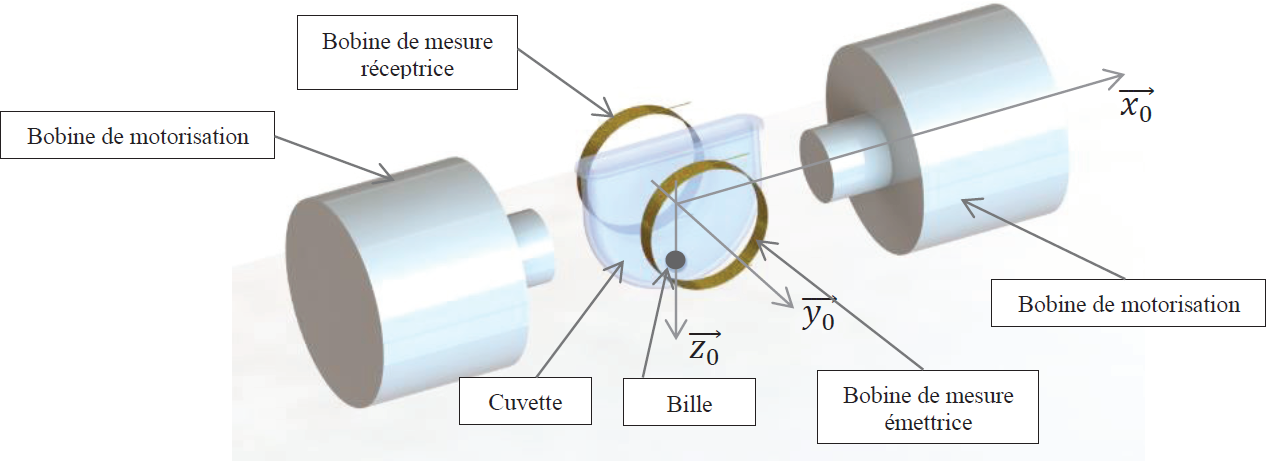
\includegraphics[width=\linewidth]{images/ccp_04}
\end{center}

La bille, roulant sans glisser sur le fond cylindrique de la cuvette, est mise en mouvement par un
champ magnétique variable induit par deux bobines motrices placées de part et d’autre de la tête de
mesure.

L’amplitude des oscillations est mesurée par deux autres bobines, l’une émettrice, l’autre réceptrice.
Après amplification du signal mesuré, on obtient un signal quasi-sinusoïdal, reflet de l’oscillation
de la bille. À viscosité constante, on obtient un balancement pendulaire constant de la bille. Quand
la viscosité augmente (phénomène de coagulation), l’amplitude d’oscillation de la bille varie.
Pour chaque mesure, le champ magnétique est ajusté en fonction de la viscosité initiale du milieu et
du type de test.



\noindent\begin{minipage}[c]{.7\linewidth}

La bille  est de masse $m$, de centre de masse $G$, de rayon $r$ et 
roule sans glisser sur un rail circulaire de rayon $R$ dans
le plan $\left( O, \vect{x_0}, \vect{y_0}\right)$. La position de la bille sur le rail est repérée par :
$\theta=\left(\vect{z_0},\vect{z_1}\right)=\left(\vect{x_0},\vect{x_1}\right)$.

$f$ est le coefficient d’adhérence au contact bille/cuvette : $f=0,1$. $J=\dfrac{2}{5}mr^2$ le moment d'inertie de la bille autour de l'axe $\axe{G}{{y_0}}$.



L'équation du mouvement de la bille est donnée par :
 $\dfrac{7}{5} m\left(R-r \right)\ddot{\theta} + f_v \left(R-r \right)\dot{\theta} + mg \sin \theta = F(t) \cos \theta$.% avec $\dot{\theta}(0)=0$ et ${\theta}(0)=0$.


\end{minipage} \hfill
\begin{minipage}[c]{.25\linewidth}
\begin{center}
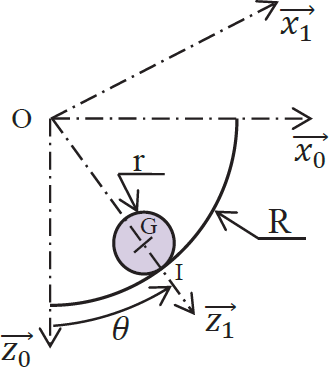
\includegraphics[width=\linewidth]{images/ccp_05}
\end{center}
\end{minipage} 


\subsubsection{Modélisation du mouvement de la bille}

\subparagraph{}\textit{$\theta$ étant petit, linéariser l’équation du mouvement puis en déduire la fonction de transfert $H(p)=\dfrac{\theta(p)}{F(p)}$. Mettre $H(p)$) sous la forme canonique d’un système du second ordre dont on donnera les expressions du gain statique $K_S$, de la pulsation propre non amortie $\omega_0$ et du
coefficient d’amortissement $\xi$ en fonction de $f_v$, $R$, $r$, $m$ et $g$.}

\subparagraph{}\textit{On prendra les valeurs numériques suivantes pour cette question :
$\omega_0 = \SI{21,8}{rad.s^{-1}}$; $K_S = \SI{25}{N^{-1}}$; $\xi=4f_v$.
Tracer, sur le document réponse****, le diagramme asymptotique de Bode en gain, ainsi que l’allure
du diagramme réel pour les valeurs suivantes du coefficient de frottement visqueux $f_v$: $f_v=0,005$, $f_v=0,05$, $f_v=0,02$.}

\subparagraph{}\textit{La sollicitation des bobines est sinusoïdale : $F(t)=F_0 \sin \left( \omega_{\text{bob}}t\right)$. Préciser, en
justifiant votre réponse, la valeur à laquelle il faut régler la pulsation $\omega_{\text{bob}}$ pour pouvoir observer, au mieux, l’évolution du coefficient de frottement $f_v$.}

\subparagraph{}\textit{Exprimer, pour un système du second ordre, en fonction de $\xi$, le rapport des amplitudes de sortie à $\omega \to 0$ et $\omega=\omega_0$ pour une même amplitude du signal d’entrée.}

\subparagraph{}\textit{Les figures suivantes représentent, avec $f_v$ constant, l’évolution de la
position de la bille $\theta$ (en degrés) en fonction du temps $t$ (en secondes)  pour différentes valeurs de pulsation $\omega_{\text{bob}}$. À partir de ces courbes et des résultats précédents, déterminer la valeur du coefficient d’amortissement $\xi$.}

\begin{minipage}[c]{.48\linewidth}
\begin{center}
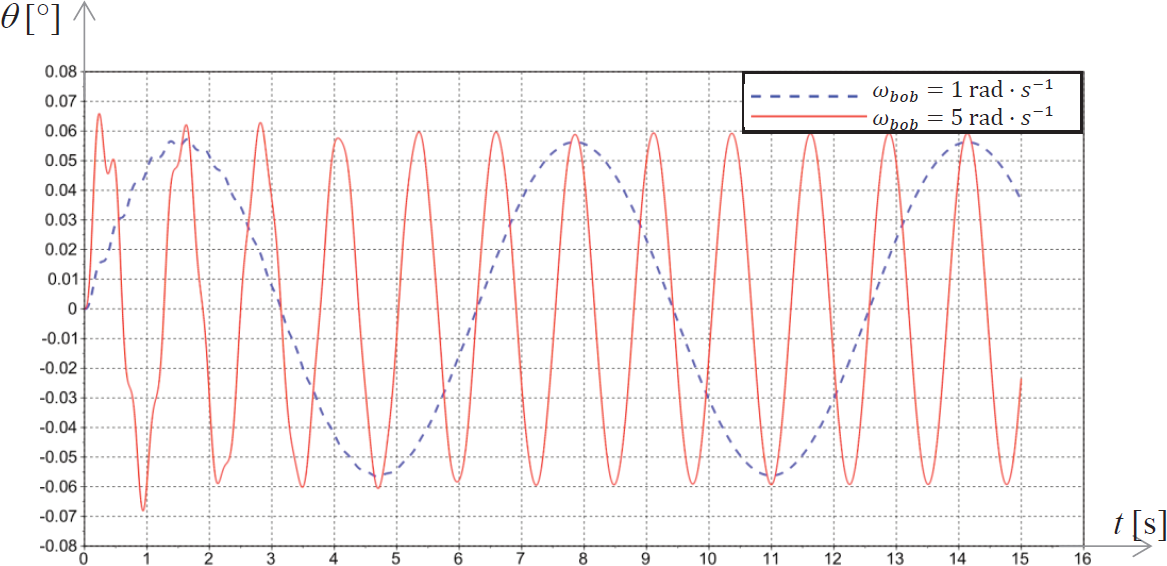
\includegraphics[width=\linewidth]{images/ccp_06}
\textit{$\theta$ en fonction de $t$  pour $\omega_{\text{bob}}= 1$ et \SI{5}{rad.s^{-1}}}
\end{center}

\begin{center}
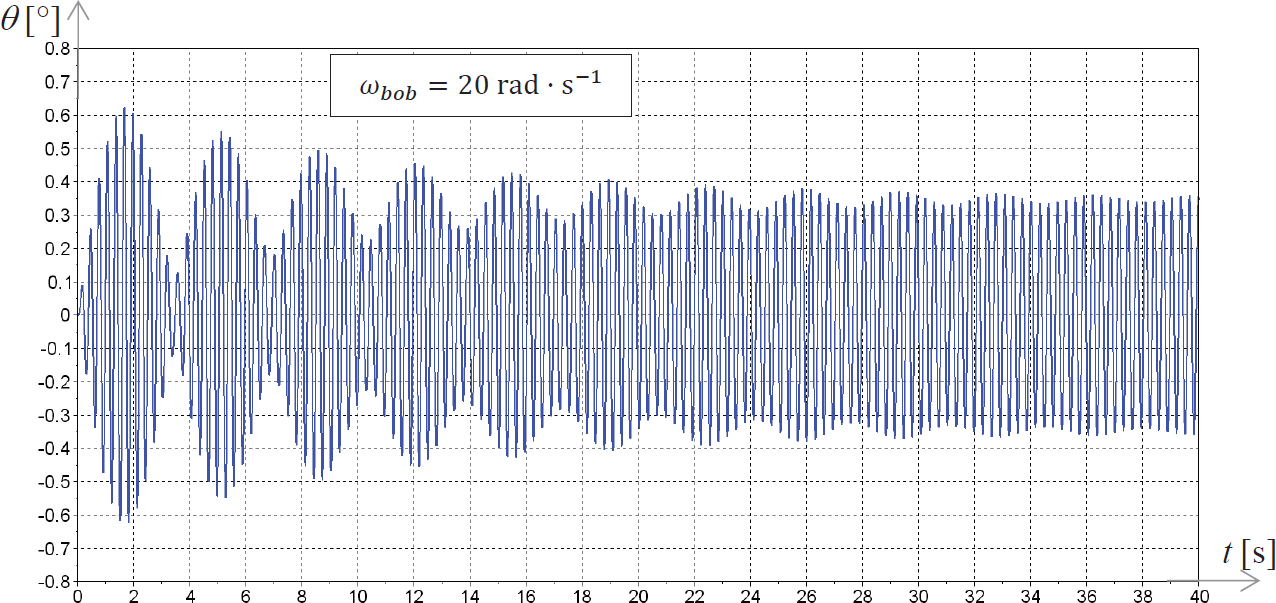
\includegraphics[width=\linewidth]{images/ccp_07}
\textit{$\theta$ en fonction de $t$  pour $\omega_{\text{bob}}= \SI{20}{rad.s^{-1}}$}
\end{center}

\end{minipage} \hfill
\begin{minipage}[c]{.48\linewidth}
\begin{center}
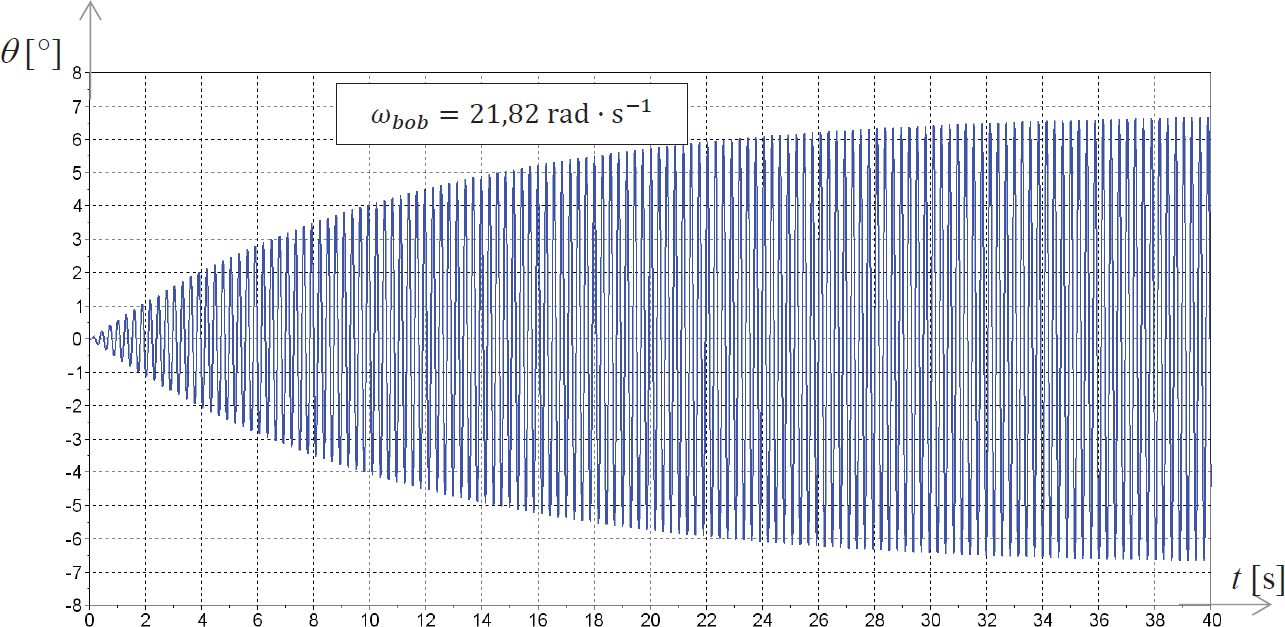
\includegraphics[width=\linewidth]{images/ccp_08}
\textit{$\theta$ en fonction de $t$  pour $\omega_{\text{bob}}= \SI{21,82}{rad.s^{-1}}$}
\end{center}

\begin{center}
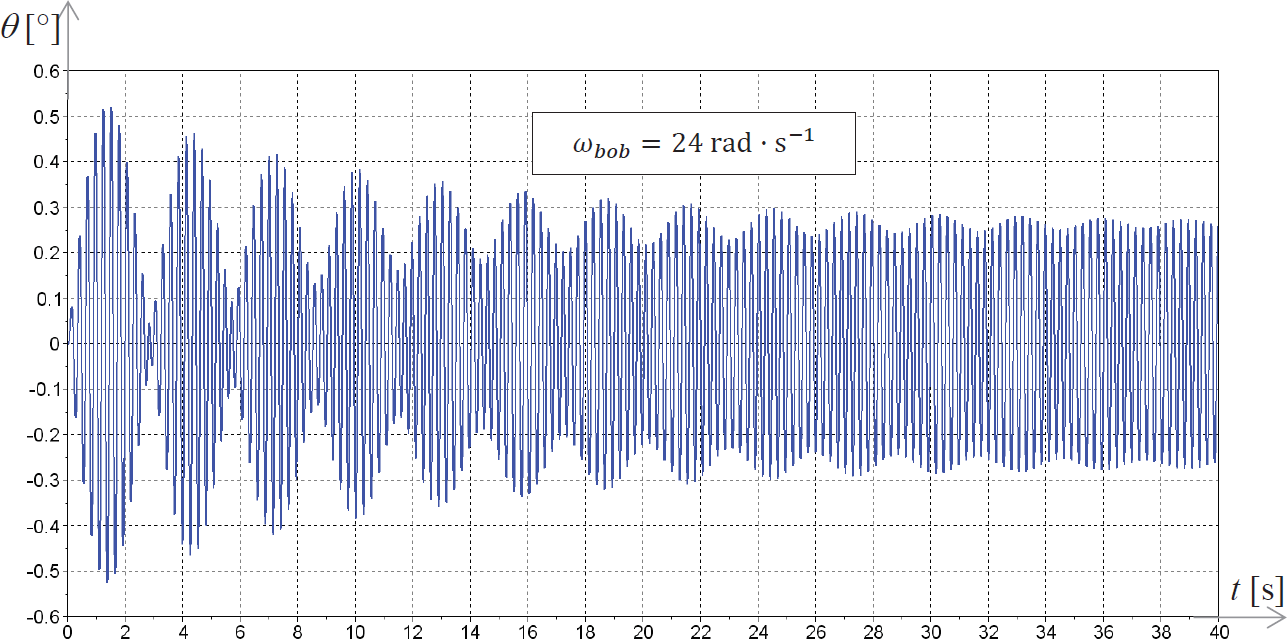
\includegraphics[width=\linewidth]{images/ccp_09}
\textit{$\theta$ en fonction de $t$  pour $\omega_{\text{bob}}= \SI{24}{rad.s^{-1}}$}
\end{center}

\end{minipage} 


\subparagraph{}\textit{En déduire la valeur numérique du coefficient de viscosité  $\eta$ du sang correspondant.}

\subparagraph{}\textit{À partir de ces analyses, en justifiant votre réponse, donner l’allure de la courbe $\theta$ en fonction de $t$ obtenue à la pulsation $\omega_0$ lorsque la viscosité du sang varie au fur et à mesure de la coagulation (si l’on suppose que $f_v$ augmente avec la coagulation).}

\subsection{Analyse de l’exigence 2.3 << Prélever les produits par déplacement suivant  $\vec{z}$ de la tête de pipetage >>}% de la tête de pipetage >>}% << Prélever les produits par le
%déplacement suivant $\vect{z}$ de la tête de pipetage >>}
\begin{obj}
Régler la commande du moteur afin de respecter le cahier des charges.
\end{obj}

\subsubsection{Présentation}
Les aiguilles de prélèvement des doses de plasma et de réactifs sont reliées à la tête de pipetage.
Elles peuvent avoir un mouvement de translation verticale (selon la direction $\vect{z}$) par rapport à cette
tête. Deux types de réactifs sont utilisés. La tête de pipetage possède donc trois aiguilles : une pour
le sang et une par type de réactif.

Successivement, pour chaque produit (plasma puis réactifs), la tête de pipetage est positionnée au dessus
du flacon approprié, l’aiguille correspondante prélève la quantité nécessaire, puis l’ensemble
tête de pipetage/aiguilles vient déposer le produit dans la cuvette d’analyse. Les aiguilles sont
ensuite plongées dans un flacon de nettoyage. L’aspiration et le refoulement des liquides (plasma et
réactifs) se font à l’aide d’une même seringue de pipetage motorisée (non représentée).

\begin{center}
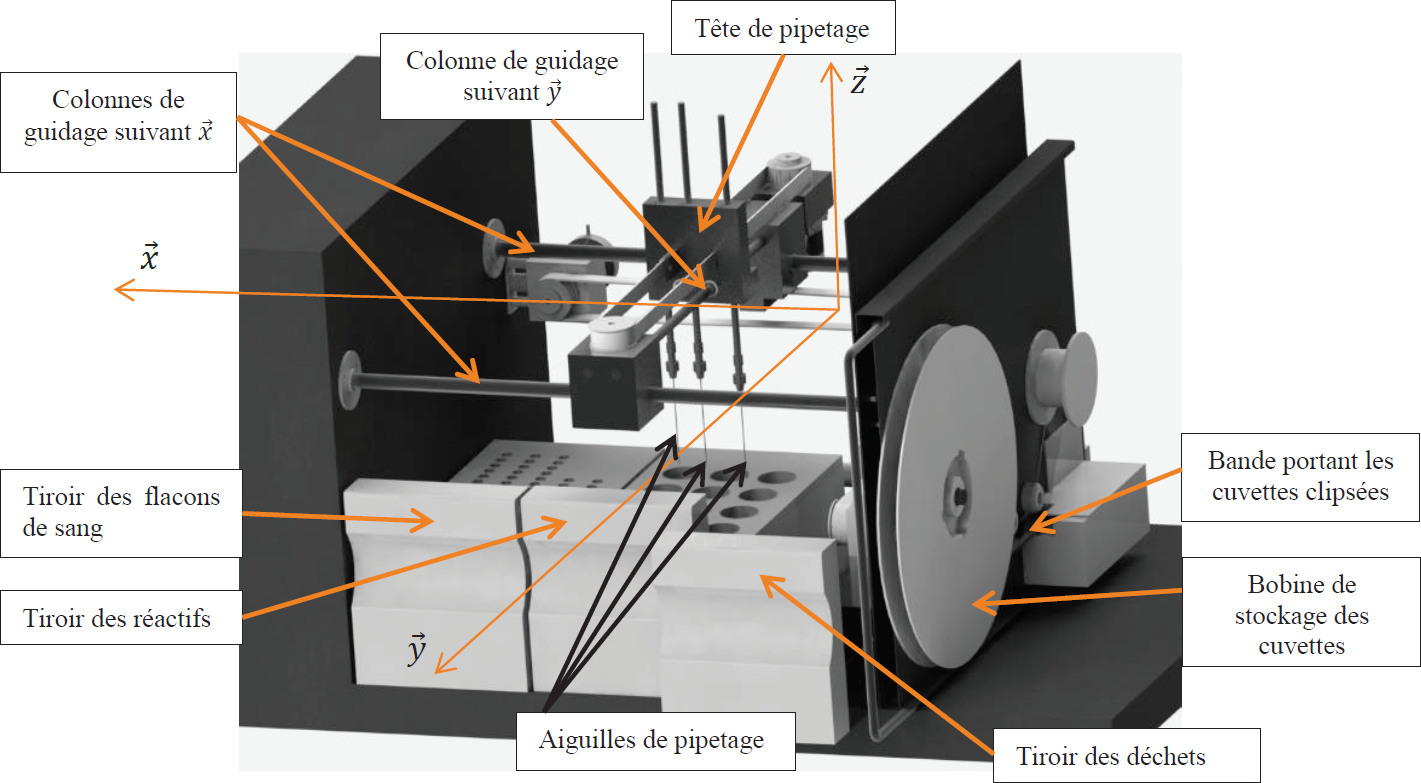
\includegraphics[width=\linewidth]{images/ccp_13}
\end{center}

\subsubsection{Modélisation de la motorisation}

Les déplacements verticaux des aiguilles de la tête de pipetage (axe $\vect{z}$) sont assurés par un ensemble motoréducteur à courant continu et système pignon-crémaillère.
On note :
\begin{itemize}
\item $ \theta_m(t)$ et $\omega_m(t)$ l’angle et la vitesse angulaire du moteur ;
\item $\omega_r(t)$ la vitesse angulaire en sortie de réducteur ;
\item $k_r=\dfrac{\omega_r}{\omega_m}=\dfrac{1}{19,2}$ le rapport de réduction du réducteur ;
\item $c_m(t)$ le couple moteur ;
\item $J_m$ l’inertie du moteur et $J_r$ l'inertie du réducteur ramenée à l’arbre moteur ;
\item $m_p = \SI{0,2}{kg}$ la masse en translation ;
\item $F_r(t) = \SI{1}{N}$ l’effort de l’opercule sur l’aiguille ;
\item $c_{\text{res}}$ couple résistant ramené à l’arbre moteur modélisant l’ensemble des frottements, y compris les frottements internes au réducteur ($c_{\text{res}}\leq 0$) ;
\item $R_p = \SI{10}{mm}$ le rayon du pignon du système pignon crémaillère ;
\item $\omega_{mn} = \SI{4 150}{tr.min^{-1}}$ la vitesse de rotation nominale du moteur ;
\item $c_{mn}= \SI{5e-3}{Nm}$ le couple moteur nominal ;
\item $E_c\left(S/Rg\right)$ l’énergie cinétique de l’ensemble $S$ par rapport au référentiel $R_g$.
\end{itemize}

L'inertie équivalente ramenée à l'arbre moteur est donnée par $J_{\text{eq}}=J_m+J_r+m_p\left(r_p k_r \right)^2$. On établit que $c_m(t)=c_r(t)+J_{\text{eq}}\dot{\omega}_m(t) \quad (4)$ avec $c_r(t)=mgR_p k_r + F_R R_pk_r - C_{\text{res}}$.



La tête de pipetage est asservie en position. Le schéma-bloc de cet asservissement est ébauché sur le
document réponse. Un codeur mesure l’angle de rotation moteur et un hacheur
module la tension aux bornes du moteur.
On note :
\begin{itemize}
\item $u(t)$ la tension aux bornes du moteur, $i(t)$ l’intensité, $e(t)$ la force électromotrice ;
\item $R$ la résistance de l’induit, $L$ son inductance, $K$ la constante de force électromotrice ;
\item $K_{\text{cod}} = \SI{2 000}{points/tr}$ le gain du codeur tel que $m_{\theta}(t) = K_{\text{cod}}\theta_m(t)$;
\item $K_\text{adap}$ le gain permettant d’adapter la consigne $z_c(t)$ à l’image de la position $m_{\theta}(t)$;
\item $H_{\text{cor}}(p)$ la fonction de transfert du correcteur ;
\item $K_h =\SI{0,094}{V.point^{-1}}$ le gain du hacheur.
\end{itemize}
Les équations du moteur à courant continu sont les suivantes :
$u(t) =Ri(t) + L\dfrac{\dd i(t)}{\dd t}+e(t) \quad (5)$, $e(t)=K\omega_m(t) \quad (6)$, $ c_m(t)=Ki(t)  \quad (7) $.

\subparagraph{}\textit{En tenant compte des notations précédentes, compléter sous forme littérale,
sur le document réponse***, le schéma-blocs de l’asservissement en position.}




\subparagraph{}\textit{Déterminer l’expression de $K_{\text{adap}}$ pour que l’écart calculé $\varepsilon$  soit proportionnel à l’erreur $z_c(t)-z(t)$.}

On note :
\begin{itemize}
\item $i_0$ l’intensité initiale ;
\item $i_{\infty}$ et $\omega_{\infty}$ l’intensité et la vitesse du moteur en régime permanent ;
\item $c_{r0}$ le couple résistant $c_{r}(t)$ supposé constant.
\end{itemize}

\subparagraph{\label{26}}\textit{Déterminer les expressions de $\left(\dfrac{\Omega_m(p)}{U(p)}\right)_{c_{r0}=0}$ et de $\left(\dfrac{I(p)}{U(p)}\right)_{c_{r0}=0}$. Mettre celles-ci
sous forme canonique.}

Afin de déterminer les caractéristiques du moteur, on applique à celui-ci un échelon de tension
($u_0(t)$) d’amplitude \SI{24}{V}. On mesure la vitesse $\omega_m(t)$ et l’intensité $i(t)$. Les résultats obtenus sont donnés sur le document réponse ********.

\subparagraph{}\textit{À partir de ces courbes et des résultats de la question \ref{26}, indiquer si l’hypothèse d’une inductance négligeable est pertinente. Justifier la réponse.}

\subparagraph{}\textit{Dans cette hypothèse d’une inductance négligeable et à partir des équations (4), (5), (6) et (7), déterminer les expressions de $i_0$, $i_{\infty}$ et $\omega_{\infty}$ en fonction de $u_0$, $c_{r0}$, $R$ et $K$.}

\subparagraph{}\textit{Déduire de cette étude les valeurs numériques de $K$ et $R$.}

\subparagraph{}\textit{Déterminer la valeur numérique du couple résistant ramené à l’arbre moteur $c_{r0}$ et de l’inertie équivalente ramenée à l’arbre moteur $J_{\text{eq}}$.}


\subsubsection{Réglage de l’asservissement}
Les résultats précédents ont permis de modéliser l’asservissement de position par le schéma-blocs ci-dessous:

\begin{center}
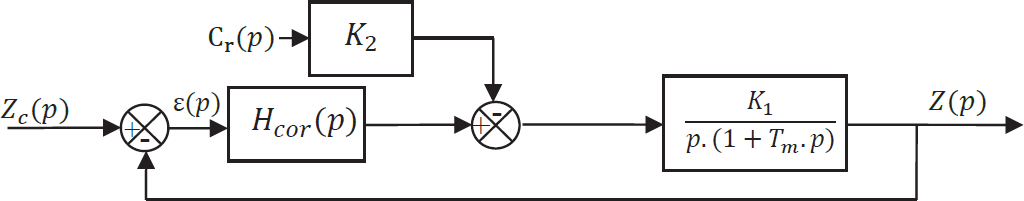
\includegraphics[width=.8\linewidth]{images/ccp_11}
\end{center}

avec $K_2 = \SI{2,78e-2}{N^{-1}}$, $K_1  = \SI{856}{s^{-1}}$, $T_m=\SI{3e-2}{s}$. Le couple résistant $C_r$ est constant et vaut $C_{r0} = \SI{2,7e-3}{Nm}$.
On suppose le correcteur proportionnel : $H_{\text{cor}}(p)=K_P$.

On donne le diagramme partiel des exigences.

\begin{center}
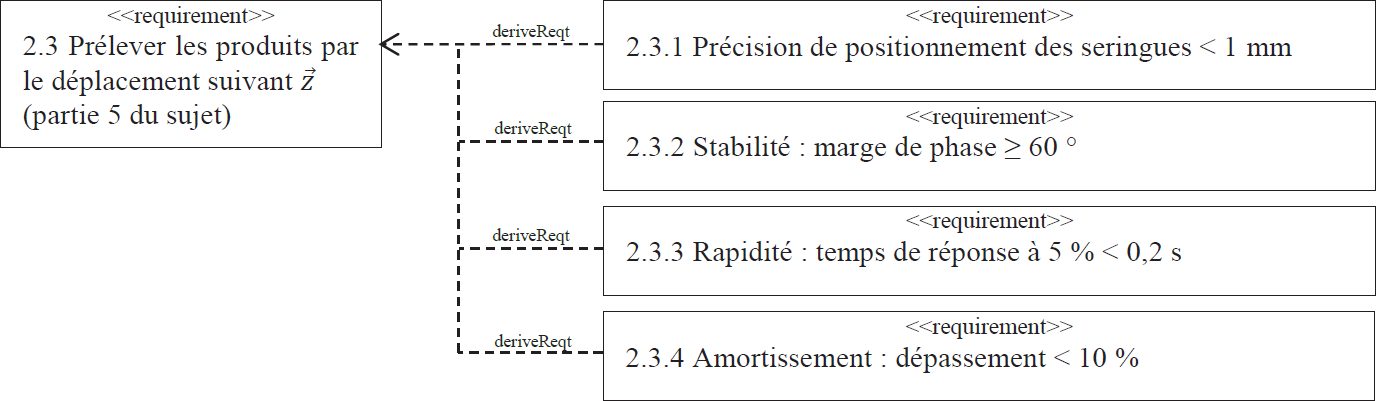
\includegraphics[width=.8\linewidth]{images/ccp_14}
\end{center}



\subparagraph{}\textit{Déterminer l’expression de la fonction de transfert en boucle ouverte $H_{\text{bo}}(p)=\dfrac{Z(p)}{\varepsilon(p)}$ ainsi que la fonction de transfert  $H_{cr}(p)=
\left(\dfrac{Z(p)}{C_r(p)}\right)_{Z_c=0}$.}


\subparagraph{}\textit{Déterminer l’erreur statique pour une entrée de type échelon d’amplitude $Z_{c0}$ dans l’hypothèse d’une perturbation nulle ($C_{r0}=0$). Déterminer ensuite l’erreur due à une
perturbation constante $C_{r0}$, définie comme la valeur finale de la position $z(t)$ dans le cas d’une
consigne de position nulle $z_c= 0$. En déduire la valeur de $K_P$ pour satisfaire le critère de
précision du cahier des charges.}

\subparagraph{}\textit{Les diagrammes de Bode en gain et en phase de $H_{bo}(p)$ sont donnés sur le document réponse pour $K_P=1$. Pour la valeur de $K_P$ déterminée précédemment, indiquer si le critère de stabilité est satisfait en justifiant votre démarche par les tracés nécessaires sur le document
réponse.}

Afin d’améliorer le comportement, on implante un correcteur Proportionnel Intégral ayant pour
fonction de transfert : $H_{\text{cor}}(p)=\dfrac{K_P\left(1+T_i p\right)}{T_i p}$ avec $K_p=1$ et $T_i=\SI{1}{s}$.
Les diagrammes de Bode de la fonction de transfert en boucle ouverte avec ce correcteur sont
donnés sur le document réponse.
On souhaite une marge de phase d’au moins 60\degres.


\subparagraph{}\textit{Justifier le choix de ce correcteur. Déterminer le coefficient $K_p$ pour satisfaire au cahier des charges. Justifier vos calculs par les tracés nécessaires sur le document réponse.****}

\subparagraph{}\textit{La figure suivante donne la réponse à un échelon de position de \SI{50}{mm} avec le correcteur précédemment réglé. Vérifier qu’elle est conforme au cahier des charges. Justifier clairement vos réponses en donnant les valeurs numériques pour chaque critère.}


\begin{center}
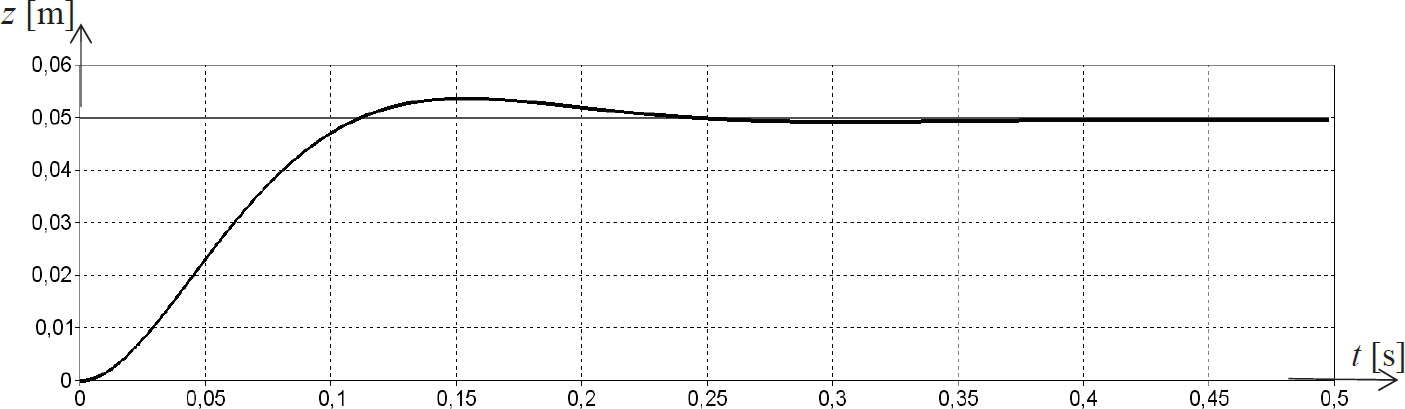
\includegraphics[width=.8\linewidth]{images/ccp_12}
\end{center}


\section{Mélangeur interne à rotors engrenant}
\subsection{Mise en situation}


\begin{minipage}[c]{.3\linewidth}
\begin{center}
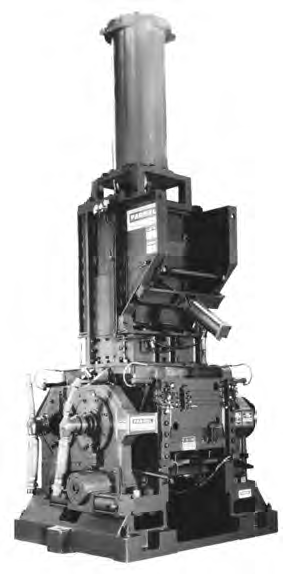
\includegraphics[width=.7\linewidth]{images/e3a_10}
\end{center}
\end{minipage}  \hfill
\begin{minipage}[c]{.65\linewidth}
Un mélangeur interne à rotors engrenants est une machine utilisée dans l'industrie pour effectuer le mélange du caoutchouc et d'additifs divers. Il est, par exemple, utilisé dans la fabrication des pneumatiques.
Nous nous intéresserons dans cette étude au modèle K5 de la société Farrel.

Le mélangeur est principalement constitué de :
\begin{itemize}
\item une porte de chargement du caoutchouc et des différents additifs (a);
\item un fouloir permettant de pousser les différents ingrédients vers la chambre de mélangeage (b);
\item deux rotors à axes parallèles tournant en sens inverses (c) et (c');
\item une chambre de mélangeage (d);
\item une porte de déchargement (e).
\end{itemize}
\end{minipage}

\begin{center}
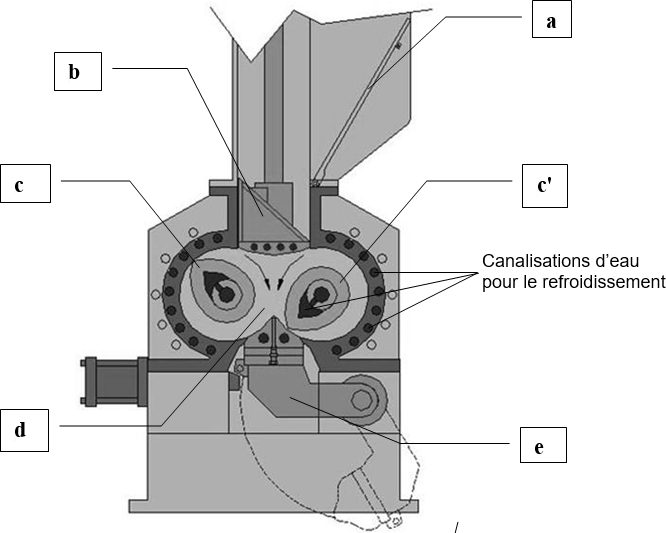
\includegraphics[width=.7\linewidth]{images/e3a_11}
\end{center}

Le modèle K5 permet de mélanger 100 kg de matière dans une chambre ayant une contenance de 143 litres. Le mélangeur a une masse totale de 16 tonnes. La masse du moteur électrique entraînant les rotors est de 2,5 tonnes.

Les caractéristiques du mélange obtenu dépendent, en plus des caractéristiques des différents constituants, des conditions dans lesquelles s'effectue le mélange. Il est donc important de maîtriser, au cours des différentes phases du mélange, la vitesse de rotation des rotors et l'effort exercé par le fouloir tout en surveillant la température dans la chambre qui ne doit pas dépasser une valeur limite (pour que le mélange ne vulcanise pas dans le mélangeur).
 




\begin{obj}
Vérifier le dimensionnement de l'actionneur. Choisir et régler un correcteur pour optimiser les performances de l'asservissement de vitesse participant à l'exigence << Effectuer le mélange dans les conditions optimales~>>.
\end{obj}



\subsection{Construction du schéma-blocs}
\begin{obj}
Mise en place de la structure globale de l’asservissement de vitesse.
\end{obj}

L'asservissement en vitesse des rotors est représenté par le schéma suivant :

\begin{center}
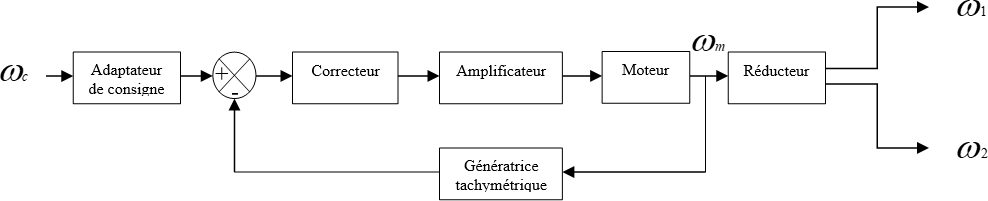
\includegraphics[width=\linewidth]{images/e3a_01}
\end{center}

$\omega_c$ : consigne de vitesse ;  $\omega_m$: vitesse moteur ; $\omega_1$: vitesse rotor 1 ; $\omega_2$ : vitesse rotor 2.

\begin{rem}
Ces quatre vitesses sont des vitesses angulaires par rapport au bâti.
\end{rem}

On donne les équations suivantes caractérisant le moteur :
\begin{multicols}{2}
\begin{enumerate}
\item $C_m(t)+C_r(t)=J\dfrac{\dd \omega_m(t)}{\dd t}$;
\item $u(t)=Ri(t)+L\dfrac{\dd i(t)}{\dd t}+e(t)$;
\item $C_m(t)=k_i i(t)$;
\item $e(t)=k_e\omega_m(t)$.
\end{enumerate}

On donne les équations suivantes caractérisant le moteur :

\begin{itemize}
\item $R$ : résistance de l'induit;
\item $L$ : inductance de l'induit;
\item $u(t)$ : tension d'alimentation du moteur;
\item $i(t)$ : courant moteur;
\item $e(t)$ : force contre électromotrice;
\item $C_m(t)$ : couple disponible sur l'arbre moteur;
\item $C_r(t)$ : couple résistant ramené sur l'arbre moteur;
\item $\omega_m(t)$ : vitesse de rotation de l'arbre moteur;
\item $J$ : moment d'inertie ramené sur l'arbre moteur;
\item $k_e$ : constante de force contre électromotrice;
\item $k_i$ : constante de couple.
\end{itemize}
\end{multicols}

On notera $C_m(p)$, $C_r(p)$, $\Omega_m(p)$, $U(p)$, $I(p)$ et $E(p)$ les transformées de Laplace des différentes grandeurs physiques définies ci-dessus.

\subparagraph{}
\textit{En considérant que toutes les conditions initiales sont nulles, donner les quatre équations précédentes dans le domaine de Laplace.}

\subparagraph{}
\textit{Remplir les fonctions de transfert des cases d, e, f et g ainsi que les trois grandeurs physiques manquantes (zones grisées) sur le schéma-bloc fourni sur le cahier réponses.}

Le schéma cinématique et les caractéristiques du réducteur sont fournis en annexe B. ****

\subparagraph{}
\textit{Donner la valeur algébrique des rapports de réduction $r_1=\dfrac{\omega_1}{\omega_m}$ et $r_2=\dfrac{\omega_2}{\omega_m}$ en fonction des nombres de dents $Z_i$. Faire les applications numériques.}

\subparagraph{}
\textit{Quelle doit être la fonction de transfert $K_a$ de l'adaptateur de consigne (case a) si l'on veut que l’écart $\varepsilon$ soit nul quand la vitesse $\omega_1$ est égale à la vitesse de consigne $\omega_c$ ? Remplir la case a du document réponse page 5****.}


Dans un premier temps nous considérerons que le correcteur est proportionnel de fonction de transfert $kc$.

\subparagraph{}
\textit{Déterminer l'expression littérale de la fonction de transfert  $H(p)=\dfrac{K}{1+\dfrac{2\xi}{\omega_0}p+\dfrac{p^2}{\omega_0^2}}$ de suivi de consigne ($C_r(p) = 0$) en fonction de $A$, $R$, $L$, $J$, $k_i$, $k_e$, $k_g$ et $k_c$. La  lettre sous la forme d'un système canonique d'ordre 2 et identifier les constantes caractéristiques.}

\subsection{Étude de l'asservissement de vitesse}

\begin{obj}
Choisir et régler un correcteur pour répondre au cahier des charges.
\end{obj}

Pour cette partie, on utilisera le schéma-blocs à retour unitaire suivant :
\begin{center}
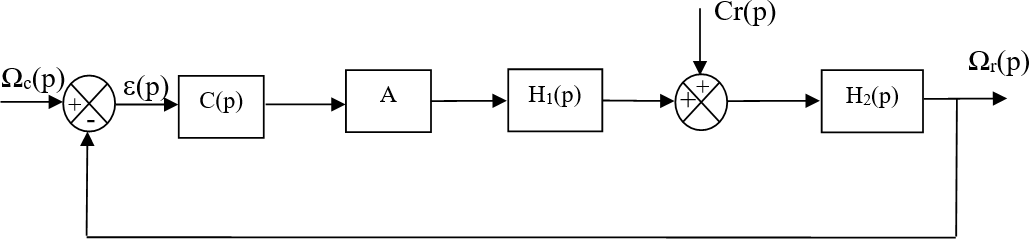
\includegraphics[width=.8\linewidth]{images/e3a_06.png}
\end{center}

On a $H_1(p)=\dfrac{3000}{1+1,6\, 10^{-2}p}$, $H_2(p)=\dfrac{5,7\, 10^{-5}\left(1+ 1,6\, 10^{-2}p\right)}{1+2,9\, 10^{-2}p+4,6\, 10^{-4}p^2}$ et $A=5$ (sans unité). Les valeurs numériques sont dans les unités du système international.

Le cahier des charges impose les conditions suivantes. 
\begin{center}
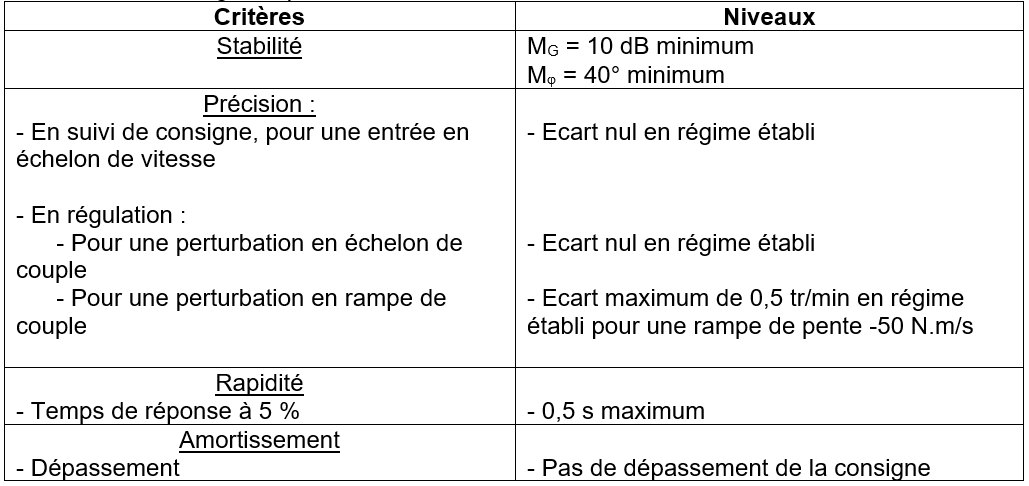
\includegraphics[width=.8\linewidth]{images/e3a_07.png}
\end{center}

\begin{rem}
\begin{itemize}
\item La perturbation en échelon de couple modélise une variation brusque du couple résistant au niveau des rotors due à la mise en action du fouloir.
\item La perturbation en rampe de couple modélise une variation lente du couple résistant liée à la variation de température du mélange.
\end{itemize}
\end{rem}

Le diagramme de Bode de la fonction de transfert en boucle ouverte du système non corrigé ($C(p) = 1$) est donné ci-dessous.

\begin{center}
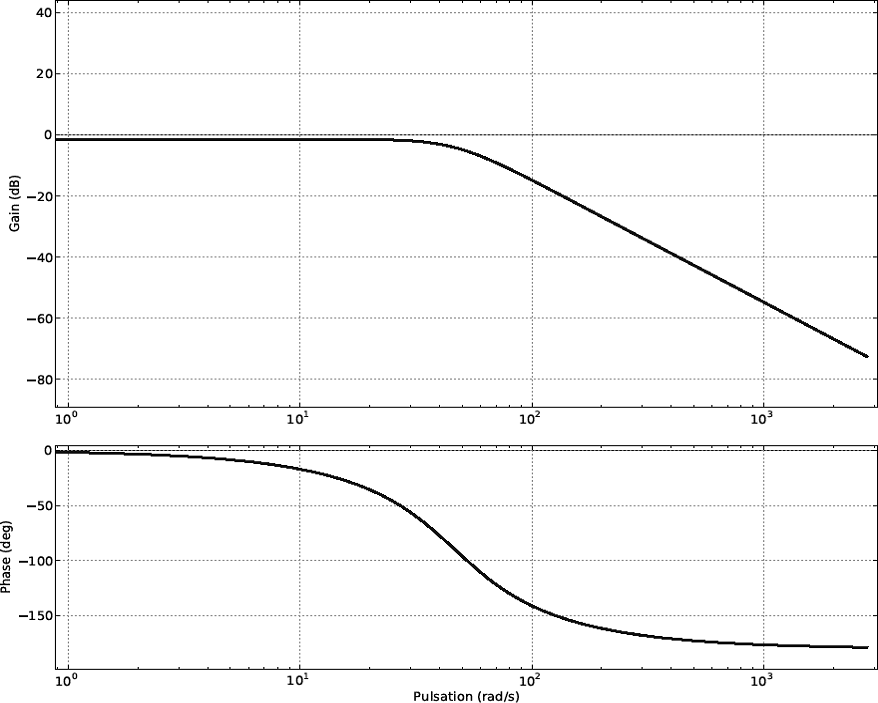
\includegraphics[width=.8\linewidth]{images/e3a_08.png}
\end{center}


\subparagraph{}
\textit{Le système modélisé ainsi est-il stable ? Justifier votre réponse.}

\subparagraph{}
\textit{Si l'on considère dans un premier temps que le correcteur est proportionnel de fonction de transfert $C(p) = K$, donner la valeur que prend l'écart (en fonction de $a$, $b$, $c$ et $K$ s’il est constant) dans chacun des trois cas proposés (on ne demande pas de développer de calculs sur la copie). Le cahier des charges est-il respecté ?}

\subparagraph{}
\textit{Parmi les quatre correcteurs proposés, cocher celui (ou ceux) qui peut (peuvent) permettre de répondre aux trois critères de précision du cahier des charges.}

\subparagraph{}
\textit{Pour la suite nous utiliserons un correcteur de fonction de transfert  $C(p)=K\dfrac{1+Tp}{Tp}$.}

\subparagraph{}
\textit{Donner le nom de ce correcteur et tracer le diagramme de Bode (asymptotique et allure du diagramme réel) du correcteur seul. Indiquer les pentes et points caractéristiques en fonction de $K$ et $T$.}

On choisit la valeur de $T$ de telle façon que la valeur de la pulsation conduisant à un déphasage de $-45\degres$ pour le correcteur seul soit dix fois plus petite que la pulsation pour laquelle la FTBO non corrigée présente un déphasage de $-90\degres$.
\subparagraph{}
\textit{Déterminer la valeur de $T$ correspondante.}

\subparagraph{}
\textit{Tracer, sur le cahier réponses, le diagramme asymptotique de Bode de la FTBO corrigée avec $K = 1$ et votre valeur de $T$. Indiquer les pentes et points caractéristiques.}

On donne, sur le cahier réponses, le diagramme de Black de la FTBO corrigée avec T déterminé à la question précédente et $K = 1$.


\subparagraph{}
\textit{Déterminer la plus grande valeur de $K$ (notée $K_{\text{stab}}$) permettant de satisfaire au critère de stabilité. Vous porterez sur la courbe les tracés que vous jugerez utiles.}

\subparagraph{}
\textit{On donne, sur le cahier réponses, les courbes de la réponse du système à une entrée en échelon unitaire ($\omega_c(t) = u(t)$) pour $K$ prenant les valeurs 1 ; 2 ; 3 ; 3,5 et 4.}


\subparagraph{}
\textit{La valeur de $K_{\text{stab}}$ trouvée à la question précédente est-elle compatible avec les critères de précision en suivi de consigne, d'amortissement et de rapidité ? Justifiez votre réponse.}

\subparagraph{}
\textit{Choisir pour $K$ une valeur permettant de respecter à la fois les critères de stabilité, amortissement, rapidité et précision en suivi de consigne. Vous justifierez vos réponses et porterez sur la courbe les tracés que vous jugerez utiles.}

 
Le correcteur ayant été dimensionné, le schéma-bloc peut se mettre sous la forme suivante :
\begin{center}
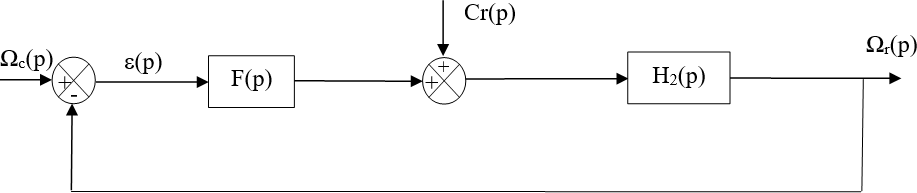
\includegraphics[width=.8\linewidth]{images/e3a_09.png}
\end{center}

On a $F(p)=\dfrac{2,25\, 10^{5}\left(1+ 10,2 p\right)}{p\left(1+1,6\, 10^{-2}p\right)}$ et $H_2(p)=\dfrac{5,7\, 10^{-5}\left(1+ 1,6\, 10^{-2}p\right)}{1+2,9\, 10^{-2}p+4,6\, 10^{-4}p^2}$. Les valeurs numériques sont dans les unités du système international.


Nous nous intéressons maintenant à la précision en régulation du système modélisé ainsi. L'étude sera donc faite pour une consigne nulle $\omega_c(t) = 0$.

\subparagraph{}
\textit{Déterminer l'expression de $\varepsilon(p)$ en fonction de $C_r(p)$, $F(p)$ et $H_2(p)$.}

\subparagraph{}
\textit{Que vaut $\varepsilon_1 = \lim\limits_{t \to + \infty} \varepsilon(t)$ pour une perturbation en échelon $C_r(t)=bu(t)$ ? Justifier votre réponse et conclure quant au respect du cahier des charges.}

\subparagraph{}
\textit{Que vaut $\varepsilon_2 = \lim\limits_{t \to + \infty} \varepsilon(t)$ pour une perturbation en rampe $C_r(t)=c t u(t)$ ? Le cahier des charges est-il respecté (justifier par l'application numérique).}

\end{document}


\begin{obj}
\end{obj}

\begin{center}
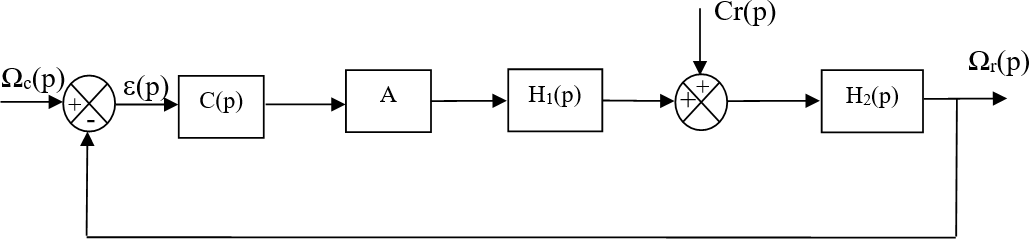
\includegraphics[width=.8\linewidth]{images/e3a_06.png}
\end{center}

\subparagraph{}
\textit{}
\ifprof
\begin{corrige}
\end{corrige}
\else
\fi
